%% abtex2-modelo-trabalho-academico.tex, v-1.7.1 laurocesar
%% Copyright 2012-2013 by abnTeX2 group at http://abntex2.googlecode.com/ 
%%
%% This work may be distributed and/or modified under the
%% conditions of the LaTeX Project Public License, either version 1.3
%% of this license or (at your option) any later version.
%% The latest version of this license is in
%%   http://www.latex-project.org/lppl.txt
%% and version 1.3 or later is part of all distributions of LaTeX
%% version 2005/12/01 or later.
%%
%% This work has the LPPL maintenance status `maintained'.
%% 
%% The Current Maintainer of this work is the abnTeX2 team, led
%% by Lauro César Araujo. Further information are available on 
%% http://abntex2.googlecode.com/
%%
%% This work consists of the files abntex2-modelo-trabalho-academico.tex,
%% abntex2-modelo-include-comandos and abntex2-modelo-references.bib
%%

% ------------------------------------------------------------------------
% ------------------------------------------------------------------------
% abnTeX2: Modelo de Trabalho Academico (tese de doutorado, dissertacao de
% mestrado e trabalhos monograficos em geral) em conformidade com 
% ABNT NBR 14724:2011: Informacao e documentacao - Trabalhos academicos -
% Apresentacao
% ------------------------------------------------------------------------
% ------------------------------------------------------------------------


%%%%%%%%%%%%%%%%%%
%
% As alterações realizadas no leiaute original do abntex2 disponibilizado 
% no sharelatex adaptaram o leiaute do abntex2 aos requisitos mínimos
% para escrita de dissertações e teses customizadas para o 
% centro de informática da ufpe.
%
% Bruno Maciel <bifm@cin.ufpe.com> 20/10/2016
%
%%%%%%%%%%%%%%%%%%%%%%%%%%%%%%%%%%%%%%%%%%%%%%%%%%%%%%%%%%%%%%%

\documentclass[
	% -- opções da classe memoir --
	12pt,				% tamanho da fonte
	openright,			% capítulos começam em pág ímpar (insere página vazia caso preciso)
	oneside,			% para impressão em verso e anverso. Oposto a oneside
	a4paper,			% tamanho do papel. 
	% -- opções da classe abntex2 --
	chapter=TITLE,		% títulos de capítulos convertidos em letras maiúsculas
	section=TITLE,		% títulos de seções convertidos em letras maiúsculas
	%subsection=TITLE,	% títulos de subseções convertidos em letras maiúsculas
	%subsubsection=TITLE,% títulos de subsubseções convertidos em letras maiúsculas
	% -- opções do pacote babel --
	%english,			% idioma adicional para hifenização
	french,				% idioma adicional para hifenização
	spanish,			% idioma adicional para hifenização
%	brazil,				% o último idioma é o principal do documento
	english,
	brazil,
	]{abntex2/abntex2}

% --
% SETTINGS

\usepackage{abntex2/abntex2-cin-ufpe}

% \usepackage[noframe]{showframe}
% \usepackage{showframe}

%\overfullrule=4mm %para identificar onde existem os alertas de linhas grandes mal formatada pelo LaTex, basta comentar para não aparecer a barra lateral preta na linha em questão.

\renewcommand*\arraystretch{1.2} %para customizar o espaço entre as linhas das tabelas


\usepackage{pdfpages} %para incluir pdf como páginas


% ---
% PACOTES
% ---
\usepackage{float}
\usepackage{cmap}				% Mapear caracteres especiais no PDF
\usepackage{lmodern}			% Usa a fonte Latin Modern			
\usepackage[T1]{fontenc}		% Selecao de codigos de fonte.
\usepackage[utf8]{inputenc}		% Codificacao do documento (conversão automática dos acentos)
\usepackage{lastpage}			% Usado pela Ficha catalográfica
\usepackage{indentfirst}		% Indenta o primeiro parágrafo de cada seção.
%\usepackage{color}				% Controle das cores
\usepackage{graphicx}			% Inclusão de gráficos
\usepackage{lipsum}				% para geração de dummy text
\usepackage[versalete,alf,abnt-and-type=e,abnt-etal-list=0,abnt-etal-cite=3]{abntex2/abntex2cite} 
\usepackage{multirow}
\usepackage[section]{placeins}



% -----------------------------------------------------------
% lista de abreviaturas e siglas
% início
% -----------------------------------------------------------
% \usepackage[noredefwarn,acronym]{glossaries} %GLOSSÁRIO
\usepackage[acronym,nonumberlist,nogroupskip,noredefwarn]{glossaries}
% \usepackage{glossary-superragged}

\newcolumntype{L}[1]{>{\raggedright\let\newline\\\arraybackslash\hspace{0pt}}m{#1}}
\newcolumntype{C}[1]{>{\centering\let\newline\\\arraybackslash\hspace{0pt}}m{#1}}
\newcolumntype{R}[1]{>{\raggedleft\let\newline\\\arraybackslash\hspace{0pt}}m{#1}}

\newglossarystyle{modsuper}{%
  \glossarystyle{super}%
  \renewcommand{\glsgroupskip}{}
  
  % put the glossary in a longtable environment:
 \renewenvironment{theglossary}%
  {
    \begin{longtable}
        {L{0.2\textwidth}L{0.8\textwidth}}}%
    {\end{longtable}
  }%
}

% -----------------------------------------------------------
% lista de abreviaturas e siglas
% fim
% -----------------------------------------------------------


\usepackage{lscape} 
\usepackage{rotating} %rotates the figures, page
\usepackage{tikz}
\usepackage[section]{placeins}
\usepackage{setspace} 



% ----------------------------------------------------------
% PERSONALIZAÇÃO DE CORES
% ----------------------------------------------------------
\definecolor{blue}{RGB}{41,5,195}
\definecolor{gray}{rgb}{.4,.4,.4}
\definecolor{gray}{rgb}{.4,.4,.4}
\definecolor{pblue}{rgb}{0.13,0.13,1}
\definecolor{pgreen}{rgb}{0,0.5,0}
\definecolor{pred}{rgb}{0.9,0,0}
\definecolor{pgrey}{rgb}{0.46,0.45,0.48}
\definecolor{lightgray}{rgb}{0.95, 0.95, 0.96}
\definecolor{whitesmoke}{rgb}{0.96, 0.96, 0.96}
\definecolor{javared}{rgb}{0.6,0,0} % for strings
\definecolor{javagreen}{rgb}{0.25,0.5,0.35} % comments
\definecolor{javapurple}{rgb}{0.5,0,0.35} % keywords
\definecolor{javadocblue}{rgb}{0.25,0.35,0.75} % javadoc
\definecolor{meucinza}{rgb}{0.5, 0.5, 0.5}
%\definecolor{lightgray}{gray}{0.9}


% ----------------------------------------------------------
% PERSONALIZAÇÃO DO USUÁRIO
% ----------------------------------------------------------

% ----------------------------------------------------------
% DADOS DO TRABALHO - CAPA e FOLHA DE ROSTO
% ----------------------------------------------------------
\titulo{\textbf{UMA LINGUAGEM ESPECÍFICA DE DOMÍNIO PARA ESPECIFICAR REGRAS DE CLASSIFICAÇÃO DE CANDIDATOS AO SISTEMA DE COTAS DA REDE DE ENSINO PÚBLICA FEDERAL}}
\autor{Daniel Severo Estrázulas}
\local{Recife}
\data{\Year}
\areaconcentracao{\textbf{Área de Concentração}: Engenharia de Software}
\orientador{\textbf{Orientador}: Leopoldo Motta Teixeira}
%\coorientador{Coorientador: Roberto Souto Maior de Barros2}
\instituicao{Universidade Federal de Pernambuco}
\departamento{Centro de Informática}
\programa{Pós-graduação em Ciência da Computação}
\emailprograma{posgraduacao@cin.ufpe.br}
\siteprograma{http://cin.ufpe.br/\textasciitilde posgraduacao}

\tipotrabalho{Dissertação de Mestrado}
% O preambulo deve conter o tipo do trabalho, o objetivo, 
% o nome da instituição e a área de concentração 
\preambulo{Trabalho apresentado ao Programa de Pós-graduação em Ciência da Computação do Centro de Informática da Universidade Federal de Pernambuco, como requisito parcial para obtenção do grau de Mestre em Ciência da Computação.}

\preambuloatadefesa{Trabalho apresentado ao Programa de Pós-Graduação em Ciência da Computação da Universidade Federal de Pernambuco, como requisito parcial para a obtenção do grau de Mestre em Ciência da Computação.}



% \renewcommand*{\acronymname}{Abreviaturas e Siglas}


\input{userlists}

% \renewcommand\partname{Part} % menu personalidado




% ----------------------------------------------------------
% COMPILA O ÍNDICE
% ----------------------------------------------------------
\makeindex
% ---


% ----------------------------------------------------------
% LISTA E ABREVIATURAS E SIGLAS
% ----------------------------------------------------------
\newacronym{MPS}{MPS}{Meta Programming System}
\newacronym{GPL}{GPL}{Linguagens de Propósito Geral}
\newacronym{DSL}{DSL}{Domain Specific Language}
\newacronym{IFSC}{IFSC}{Instituto Federal de Santa Catarina}
\newacronym{DTIC}{DTIC}{Diretoria de Tecnologia da Informação e Comunicação}
\newacronym{MEC}{MEC}{Ministério da Educação}
\newacronym{JOVIAL}{JOVIAL}{Jules Own Version of the International Algorithmic Language}
\newacronym{MVC}{MVC}{Model View Controller}
\newacronym{IBGE}{IBGE}{Instituto Brasileiro de Geografia e Estatística}
\newacronym{ENEM}{ENEM}{Exame Nacional do Ensino Médio}
\newacronym{SISU}{SISU}{Sistema de Seleção Unificada}
\newacronym{PCD}{PCD}{Pessoas Com Deficiência}
\newacronym{PPI}{PPI}{Candidatos autodeclarados Pretos, Pardos ou Indígenas}
\newacronym{SERES}{SERES}{Secretaria de Regulação e Supervisão da Educação Superior}
\newacronym{IDE}{IDE}{Integrated Development Environment}
\newacronym{AST}{AST}{Árvore de Sintaxe Abstrata}
\newacronym{XML}{XML}{Extensible Markup Language}
\newacronym{BNF}{BNF}{Backus Naur Form}
\newacronym{EMF}{EMF}{Eclipse Modeling Framework}
\newacronym{SDF}{SDF}{Syntax Definition Formalism}

\makenoidxglossaries
\renewcommand*{\glsseeformat}[3][\seename]{\textit{#1}  
\glsseelist{#2}}

\renewcommand*{\glspostdescription}{} % remove trailing dot
\renewcommand{\glsnamefont}[1]{\textbf{#1}}

\renewcommand{\familydefault}{\sfdefault}

% ----------------------------------------------------------
% GLOSSÁRIO
% ----------------------------------------------------------




\newglossaryentry{naive-bayes}
{
  name=\textit{Na{\"i}ve Bayes},
  description={},
  plural=\textit{Na{\"i}ve Bayes}
}

\newglossaryentry{hoeffding-tree}
{
  name=\textit{Hoeffding Tree},
  description={},
  plural=\textit{Hoeffding Trees}
}


















\usepackage{inconsolata}
\usepackage{listings}

\lstset{language=Java,
basicstyle=\ttfamily\scriptsize,
%basicstyle=\ttfamily,
keywordstyle=\color{javapurple}\bfseries,
stringstyle=\color{pblue},
commentstyle=\color{javagreen},
morecomment=[s][\color{javadocblue}]{/**}{*/},
morecomment=[s][\color{gray}]{@}{\ },
numbers=left,
numberstyle=\tiny\color{black},
stepnumber=2,
numbersep=8pt,
tabsize=4,
showspaces=false,
showstringspaces=false,
breaklines=true,}

%%%%%%%%%%%%%%%%%%%%%%%%%%%%%%%%%%




\usepackage{adjustbox} % ajustar tabela ao tamanho da pagina


% ----------------------------------------------------------
% INÍCIO DO DOCUMENTO
% ----------------------------------------------------------
\begin{document}

\frenchspacing % Retira espaço extra obsoleto entre as frases.

\imprimircapa
\imprimirfolhaderosto*~
%\newpage
% \thispagestyle{empty}
% \null
% \vfill
% \begin{flushbottom}
% 	\begin{center}
%     \centering
%         Catalogação da fonte\par
%         Bibliotecária Jane Souto Maior, CRB4-571
% 		\fbox{
%             \begin{minipage}[t][7.5cm][t]{12cm} 
%                 \hspace{1.5em}
%                     M152w \setlength{\parindent}{0.7cm} Maciel, Bruno Iran Ferreira \setlength{\parindent}{0.7cm}\par
% {\imprimirtipotrabalho} / {\imprimirautor}. - Recife: O Autor, {\imprimirdata}.\par 
% 114 .: fig., tab.\par
% {\imprimirorientador}.\par
% {\imprimirtipotrabalho} – {\imprimirinstituicao}. CIn. Ciência da computação, {\imprimirdata}.\newline Inclui referências e apêndice.\par
% 1. Banco de Dados 2. Web semântica. I. Lóscio, Bernadette Farias (orientadora). II. Título.
% 025.04              CDD (23. ed.)          UFPE- MEI 2015-188
% 		    \end{minipage}
% 		    }
% 	\end{center}	
% \end{flushbottom}

%se for arquivo em pdf basta usar a tag abaixo


\includepdf[pages=-]{appendix/ficha.pdf}

%\newpage
%
\thispagestyle{empty}
\begin{center}

    %\vspace*{1cm}
    \textbf{{\ABNTEXchapterfont\fontsize{12}{12}\selectfont\imprimirautor}}
	
    \vspace{2cm}
    \begin{center}
      \ABNTEXchapterfont\fontsize{12}{12}\selectfont\imprimirtitulo
    \end{center}
    \vspace{0.5cm}
	

      \hspace{.20\textwidth}
      \begin{minipage}{.55\textwidth}
      	\SingleSpacing
         \imprimirpreambuloatadefesa
       \end{minipage}%
       
    \vspace{0.5cm}
    \begin{flushleft}
    {\fontsize{12}{12}\selectfont Aprovado em: 04/09/2020.}
    \vspace{0.5cm}
    %\par\noindent\rule{0.6\textwidth}{0.4pt}\\
    %{\bfseries\fontsize{12}{12}\selectfont\imprimirorientador\par}
    \end{flushleft}

     \vspace{1cm}
     
    {\bfseries\fontsize{12}{12}\selectfont\ BANCA EXAMINADORA}
    
    \vspace{1cm}
    
        % \tikz\draw (0,0) -- (11,0);\\
        
		{\SingleSpacing
		\par\noindent\rule{0.6\textwidth}{0.4pt}\\
		Prof. Leopoldo Motta Teixeira\\
		Centro de Informática / UFPE}
        
        \vspace{0.2cm}
        {\SingleSpacing
		\par\noindent\rule{0.6\textwidth}{0.4pt}\\
		Prof. Márcio Lopes Cornélio\\
		Centro de Informática / UFPE}
		
        \vspace{0.2cm}
        {\SingleSpacing
		\par\noindent\rule{0.6\textwidth}{0.4pt}\\
		Prof. Elder de Macedo Rodrigues\\
		Universidade Federal do Pampa / UNIPAMPA}
		
	
  \end{center}
  
  

% %\newpage
% \thispagestyle{empty}

% \normalfont\normalsize

% \noindent
% {\imprimirtipotrabalho} apresentada por \textbf{{\imprimirautor}} à Pós-Graduação em Ciência da Computação do Centro de Informática da Universidade Federal de Pernambuco, sob o título ``\textbf{\imprimirtitulo}'' %orientador:
% \textbf{\imprimirorientador} e aprovada pela Banca Examinadora formada pelos professores:
% \vfill

% \begin{center}
   
%   \vspace{2cm}
   
% \begin{flushright}


% 		\tikz\draw (0,0) -- (11,0);\\
% 		\vspace{0.1cm}
% 		\begin{minipage}{110mm}
% 	%	\quotefonti
% 		Prof. XX%Kiev Santos Gama\\
% 		Centro de Informática/ UFPE\\
% 		%\vspace{1cm}
% 		\end{minipage}
% 		\vfill
% 	%\vspace*{0.9cm}
%         \tikz\draw (0,0) -- (11,0);\\
%         \vspace{0.1cm}%\vspace{\stretch{0.1}}

% 		\begin{minipage}{110mm}
% 	%	\quotefonti
% 		Profa. YY%Damires Yluska de Souza Fernandes\\
% 		Gerência Educacional de Informática / IFPB\\
		
% 		%\vspace{1cm}
% 		\end{minipage}
% 		\vfill
		
% 		\tikz\draw (0,0) -- (11,0);\\
% 		\vspace{0.1cm}%\vspace{\stretch{0.1}}
% 		\begin{minipage}{110mm}
% 		%\quotefonti		
% 		Profa. TT%Bernadette Farias Lóscio\\
% 		Centro de Informática / UFPE\\
% 		\end{minipage}
		

		
% 		\vfill
% 		\tikz\draw (0,0) -- (11,0);\\
% 		\vspace{0.1cm}%\vspace{\stretch{0.1}}
% 		\begin{minipage}{110mm}
% 		%\quotefonti		
% 		Prof. {\imprimirorientador}\\
% 		Centro de Informática / UFPE\\
% 		\end{minipage}
		
		
% \end{flushright}

% \end{center}

%  \vspace*{\fill}
% \begin{flushleft}
% 	\vfill
	
% 	\vfill
% 	Visto e permitida a impressão.
	
% 	Recife, 2 de Julho de {\imprimirdata}.
% 	\vfill
	
% 	\vspace{1cm}
	
% 	\tikz\draw (0,0) -- (11,0);\\
% 	\textbf{Prof. Ricardo Bastos Cavalcante Prudêncio}\\
% 	Coordenadora da Pós-Graduação em Ciência da Computação do\\{\tiny }
% 	Centro de Informática da Universidade Federal de Pernambuco.
% \end{flushleft}

% \newpage
% % ----------------------------------------------------------
% DEDICATÓRIA
% ----------------------------------------------------------
\begin{dedicatoria}
   \vspace*{\fill}
%   \centering
   \noindent
   \textit{\lipsum[2]} 
   %\vspace*{\fill}
\end{dedicatoria}
% ---

% ----------------------------------------------------------
% AGRADECIMENTOS
% ----------------------------------------------------------
\begin{agradecimentos}
Ao Programa de Pós-Graduação em Ciência da Computação do Centro de Informática da Universidade Federal de Pernambuco, em nome do Coordenador Professor \textbf{Ricardo Bastos Cavalcante Prudêncio}.

Ao Orientador Professor \textbf{Leopoldo Motta Teixeira}, pela paciência, por contribuir com os conhecimentos sobre o tema alvo da pesquisa, assim como as suas valiosas contribuições no desenvolvimento do trabalho.

Aos Professores \textbf{Marcio Lopes Cornelio} e \textbf{Vanilson André de Arruda Buregio} pelas contribuições na Banca de Qualificação.

A minha mãe, \textbf{Julia Rosa Severo}, pelo apoio e pela motivação durante o meu processo estudantil e acadêmico.

A minha esposa, \textbf{Ana Paula Boff}, pela compreensão e pelo apoio durante as minhas ausências necessárias para o acompanhamento das aulas e para o desenvolvimento desse estudo.

Aos colegas \textbf{Eliandro Luiz Minski} e \textbf{Samuel Bristot Loli}, pela parceria durante as atividades do curso, assim como pela troca de conhecimentos e experiências de vida que vão contribuir de maneira imensurável para o meu futuro profissional e pessoal.

Ao \textbf{IFSC} pela oportunidade e liberação para as aulas, aos colegas da \textbf{Reitoria}, em especial os amigos da \textbf{DTIC}, pela troca de ideias, dicas, sugestões e pelo apoio nos compromissos e atividades assumidas em função da minha ausência durante as aulas.

A todos os \textbf{Professores}, \textbf{Técnicos Administrativos} e \textbf{Auxiliares} do \textbf{CIN}, em especial, a servidora \textbf{Joelma Souza de Menezes Franca} que sempre nos atendeu com presteza e prontidão em todos os assuntos e solicitações relativas ao curso.

A \textbf{todos os colegas de aula}, que contribuíram para os trabalhos em grupo, discussões, estudos e risadas durante as atividades realizadas dentro e fora do câmpus. 




\end{agradecimentos}
%

% ----------------------------------------------------------
% EPÍGRAFE
% ----------------------------------------------------------
\begin{epigrafe}
    \vspace*{\fill}
	\begin{flushright}
		\textit{A bravata não é sinônimo de bravura. A bravata e a violência são uma questão menos de forma que de espírito. O homem bravo é consciente de seus deveres e da justiça. Sabe bater-se pelas ideias fazendo dos obstáculos não uma respectiva derrota, mas sim um fator estímulo. Gichin Funakoshi}
	\end{flushright}
\end{epigrafe}

% resumo em português
\begin{resumo}[Resumo] \noindent 
Este trabalho apresenta uma pesquisa que tem como objetivo compreender, por meio da elaboração de uma linguagem específica de domínio, a viabilidade de melhoria na comunicação entre usuários de negócio e desenvolvedores, visando o aumento na produtividade da especificação de requisitos e da implementação de regras concernentes ao sistema de cotas da rede de ensino pública federal. A classificação de candidatos cotistas é garantida por meio da lei Nº 12.711/2012, em conjunto com os decretos Nº 7.824 e Nº 9.034, os quais passaram por mudanças em suas diretrizes nos anos de 2012, 2016 e 2017. Adicionalmente a essas mudanças, podem ocorrer situações em que a interpretação de lei é alterada. Essas dificuldades podem resultar em atrasos na aderência à legislação, assim como falhas na comunicação entre desenvolvedores e especialistas de negócio. Portanto, a criação de uma linguagem que expresse regras de distribuição de vagas de maneira mais clara poderá auxiliar na geração de código de classificação com menor dependência de conhecimento técnico em programação, o que pode contribuir para a celeridade dos processos de ingresso em futuras alterações de regras de classificação. Como metodologia realizou-se uma pesquisa de natureza qualitativa com 20 usuários, de modo a verificar as dificuldades de compreensão e uso da linguagem desenvolvida na ferramenta Meta Programming System (MPS) da JetBrains, além do desenvolvimento de uma \gls{API} como prova de conceito para a respectiva geração do serviço de classificação. Para tanto, esse trabalho foi baseado em um levantamento do histórico de mudanças no sistema de controle de versões do \gls{IFSC}, no qual foram identificadas as principais alterações realizadas em função de versões de lei até o momento. Como resultado da presente pesquisa obteve-se o comparativo de dificuldades e preocupações sobre o uso da DSL entre 4 (quatro) grupos de usuários com diferentes características de formação e experiência. Após essa análise foram implementadas algumas melhorias na linguagem, com relação aos comentários e sugestões dos usuários. Ademais, com os testes da \gls{API}, foi possível comparar os resultados da implementação da linguagem com os dados históricos de processamento de candidatos do IFSC em 16 processos seletivos. Por fim, conclui-se que a aplicação da DSL Cotas pode contribuir para a melhoria de comunicação e de entendimento entre os diferentes perfis de conhecimento dos envolvidos, além de propor um novo meio de aplicação prática-teoria de linguagens de domínio específicas. Ressalta-se a relevância social desse estudo, no que diz respeito às ações institucionais para atendimento de demandas que tratam de questões sobre a inclusão social como prioridade nos processos seletivos de ingresso.

% \noindent %- o resumo deve ter apenas 1 parágrafo e sem recuo de texto na primeira linha, essa tag remove o recuo. Não pode haver quebra de linha.

 \vspace{\onelineskip}
    
 \noindent
 \textbf{Palavras-chaves}: Linguagem de Domínio Específico. Meta Programming System. Lei de Cotas 12.711/2012. Regras para Classificação de Candidatos. Rede Federal de Ensino.
\end{resumo}



% resumo em inglês
\begin{resumo}[Abstract]
\begin{otherlanguage*}{english}

 \noindent
\lipsum[5]

   \vspace{\onelineskip}
 
   \noindent 
   \textbf{Key-words}: Domain Specific Language. Meta Programming System. Vacancy Reservation Law 12.711/2012.
 \end{otherlanguage*}
 \end{resumo}



% ----------------------------------------------------------
% LISTA DE FIGURAS
% ----------------------------------------------------------
\pdfbookmark[0]{\listfigurename}{lof}
\listoffigures*
\cleardoublepage


% ----------------------------------------------------------
% LISTA DE TABELAS
% ----------------------------------------------------------

\pdfbookmark[0]{\listtablename}{lot}
\listoftables*
\cleardoublepage

% ---
% LISTA DE CÓDIGOS FONTES
% ---

\pdfbookmark[0]{\lstlistingname}{lol} % caso não tenha quadros, comente esta linha 
\counterwithout{lstlisting}{chapter}


% Altera o nome padrão do rótulo usado no comando \autoref{}
\renewcommand{\lstlistingname}{Código Fonte}

% Altera o rótulo a ser usando no elemento pré-textual "Lista de código"
\renewcommand{\lstlistlistingname}{Lista de códigos}

% Configura a ``Lista de Códigos'' conforme as regras da ABNT (para abnTeX2)
\begingroup\makeatletter
\let\newcounter\@gobble\let\setcounter\@gobbletwo
  \globaldefs\@ne \let\c@loldepth\@ne
  \newlistof{listings}{lol}{\lstlistlistingname}
  \newlistentry{lstlisting}{lol}{0}
\endgroup

\renewcommand{\cftlstlistingaftersnum}{\hfill--\hfil}

\let\oldlstlistoflistings\lstlistoflistings
{
\let\oldnumberline\numberline
\newcommand{\algnumberline}[1]{Código Fonte~#1~\enspace--~\enspace}
\renewcommand{\numberline}{\algnumberline}

\begin{KeepFromToc}
\lstlistoflistings
\end{KeepFromToc}
}
\cleardoublepage


        
  
% ----------------------------------------------------------
% LISTA E ABREVIATURAS E SIGLAS
% ----------------------------------------------------------
% \printglossary[type=\acronymtype,title={\listadesiglasname},nonumberlist]
% \printglossaries
% compile uma vez com o comando \printglossaries e depois compile novamente com o comando \printglossaries comentado para as páginas glossário e siglas serem ocultadas.

% ----------------------------------------------------------
% LISTA E ABREVIATURAS E SIGLAS
% ----------------------------------------------------------
% \setglossarystyle{modsuper}
\printnoidxglossary[style=modsuper,type=\acronymtype,title={\listadesiglasname},nonumberlist]
% \printglossary[style=super, type=\acronymtype]
\cleardoublepage



% ----------------------------------------------------------
% LISTA DE SIMBOLOS


% ----------------------------------------------------------
%


% ---

% ---
% inserir lista de símbolos
% ---
\begin{simbolos}
 %\item[$ \gamma $] Letra grega Gama
  %\item[$ \Lambda $] Lambda
  %\item[$ \zeta $] Letra grega minúscula zeta
  %\item[$ \in $] Pertence
%  \item[$ \infty$] Infinito
%  \item[$ \ge$] Maior ou Igual
  %\item[$ \delta$] Delta
  %\item[$ \theta$] Teta
  %\item[$ \sigma$] Sigma
  \item[$ \mu$] Mi
  
\end{simbolos}
% ---






% ----------------------------------------------------------
% SUMÁRIO
% ----------------------------------------------------------
\pdfbookmark[0]{\contentsname}{toc}
\tableofcontents*
% \begingroup\intoctrue
% \tableofcontents*
% \endgroup
\cleardoublepage

% \setcounter{page}{13}
\setcounter{tocdepth}{2}
\setcounter{table}{0}




% ----------------------------------------------------------
% ELEMENTOS TEXTUAIS
% ----------------------------------------------------------
\textual



  \chapter{Introdução}
\label{chap:intro}

Este capítulo apresenta a organização do trabalho e contextualiza a justificativa e a relevância sobre o tema desta dissertação. 

 \section{Organização do trabalho}
\label{organizacao}

O presente trabalho é organizado nos seguintes capítulos:

\begin{itemize}
    \item Capítulo \ref{chap:intro}: Introdução - que apresenta a motivação, a contextualização, os objetivos e a organização do trabalho;
    \item Capítulo \ref{chap:historicoversoes}: Sistema de Ingresso e Versionamento - que elenca o histórico de mudanças no sistema de cotas do sistema de ingresso do \gls{IFSC}, o que motivou o estudo inicial desta pesquisa;
    
    \item Capítulo \ref{chap:fundamentacao}: Fundamentação Teórica - o qual aborda a revisão da literatura sobre os temas ligados ao desenvolvimento de \gls{DSL} na engenharia de software, as diferenças sobre \gls{GPL}, as vantagens e desvantagens do uso  \gls{DSL}, assim como as ferramentas utilizadas para a sua construção;
        
    \item Capítulo \ref{metodologia}: Metodologia - no qual é descrita a classificação e as etapas da pesquisa, o ambiente da pesquisa e os métodos de avaliação da DSL;

    \item Capítulo \ref{chap:dslcotas}: DSL de Cotas - que aborda uma \gls{DSL} como meio de simplificar a especificação e desenvolvimento de regras de classificação de candidatos ao sistema de cotas da rede de ensino pública federal, assim como apresenta a \gls{API} DSL Cotas, responsável por implementar o serviço de classificação e aprovação de candidatos;
    \item Capítulo \ref{chap:analise}: Avaliação e Análise dos Resultados - o qual contém a análise dos dados coletados por meio de um exercício prático de avaliação da DSL Cotas, de um questionário aplicado com os usuários e da avaliação da
    \gls{API} DSL Cotas;
    \item Capítulo \ref{chap:consideracoes}: Conclusões - na qual é realizada uma síntese dos principais resultados da pesquisa, bem como os trabalhos relacionados, o espoco negativo da pesquisa, as principais contribuições da DSL Cotas, os trabalhos futuros sugeridos e as considerações finais.
\end{itemize}


Nas seções \ref{contextualizacao} e \ref{motivacao} serão abordados os elementos contextuais e motivacionais para desenvolvimento desse estudo, enquanto nas seções \ref{problema} e \ref{objetivos} serão apontados o problema, as hipóteses e os objetivos da pesquisa. Por fim, na seção \ref{metodologia} serão definidos os métodos utilizados.


 \section{Contextualização}
\label{contextualizacao}

 Para \citeonline{ghosh2011dsl}, problemas na comunicação entre desenvolvedores e especialistas de domínio são os principais motivos de falha no desenvolvimento e evolução de projetos de software. Especialistas, entendem a terminologia do domínio e falam em um vocabulário que pode ser estranho para as equipes de desenvolvedores. Nesse sentido, é preciso identificar meios para redução da lacuna semântica entre especialistas e desenvolvedores, de modo que os especialistas possam estar envolvidos na verificação de regras de negócio ao longo do ciclo de vida do projeto.

 A constante alteração de regras de negócio advém de mudanças de lei, forças de mercado ou novos objetivos empresariais, exigindo que essas possam ser expressas de modo a serem compreendidas e facilmente alteradas pelas organizações, a fim de melhorar o desempenho de negócios \cite{flexiblerules}.
 
 Segundo \citeonline{verificationbusinessrules}, a mudança de regras de negócio é inevitável, sendo cada vez mais frequente a adaptação às novas regulamentações e a necessidade de os sistemas estarem em conformidade com novas regras, que por décadas são implementadas em softwares de áreas industriais, financeiras, empresas de seguros, administração e várias outras.
 
 O \gls{IFSC} é uma instituição da rede de ensino pública federal presente no estado de Santa Catarina há mais de 100 anos, que hoje desenvolve e mantém diversos sistemas de informação, os quais estão sujeitos a alterações para conformidade à legislação federal. As aplicações institucionais têm como principais envolvidos os discentes, os professores e os técnicos administrativos, que participam da oferta de cursos nos mais diversos níveis, tais como cursos de qualificação profissional, educação jovens e adultos, técnicos, superiores e pós-graduação. 
 
 Ao que concerne à necessidade de adaptação a novas regras de negócio, o autor da presente pesquisa trata sobre um dos sistemas de informação mais utilizados internamente, o sistema de ingresso de discentes na instituição, o qual é mantido desde 2007 pela \gls{DTIC} e tem como objetivo disponibilizar ofertas de vagas em cursos por meio de processos seletivos. Atualmente, a base de dados do sistema conta com 788 processos seletivos e mais de 409 mil registros de candidatos.
 
 A principal funcionalidade do sistema de ingresso do \gls{IFSC} é a classificação de candidatos, a qual é construída e mantida conforme critérios da Lei nº 12.711/2012, que estabelece:
 \begin{citacao}
 Art. 1º As instituições federais de educação superior vinculadas ao Ministério da Educação reservarão, em cada concurso seletivo para ingresso nos cursos de graduação, por curso e turno, no mínimo 50\% (cinquenta por cento) de suas vagas para estudantes que tenham cursado integralmente o ensino médio em escolas públicas.
 
 Art. 3º Em cada instituição federal de ensino superior, as vagas de que trata o art. 1º desta Lei serão preenchidas, por curso e turno, por autodeclarados pretos, pardos e indígenas e por pessoas com deficiência, nos termos da legislação, em proporção ao total de vagas no mínimo igual à proporção respectiva de pretos, pardos, indígenas e pessoas com deficiência na população da unidade da Federação onde está instalada a instituição, segundo o último censo da Fundação Instituto Brasileiro de Geografia e Estatística - IBGE \cite{leicotas}.  
 \end{citacao}
 
 A adequação à legislação é demanda proveniente do \gls{MEC}, o qual faz referência em seu site aos decretos nº 7.824/2012, nº 9.034/2017 (que regulamentam a lei nº12.711) e às portarias normativas nº 18/2012 e nº 9/2017, as quais estabelecem regras, conceitos básicos e fórmulas para preenchimento das modalidades de reservas de vagas do sistema de cotas. 
 
 Sempre que o \gls{MEC} realiza alterações em um dos documentos de lei citados, é necessário também alterar os sistemas de informações das instituições de ensino. A exigência para adequação dos sistemas à lei traz o aumento da demanda de desenvolvimento, situação ilustrada no Capítulo  \ref{chap:historicoversoes}, no qual é elencado o histórico do controle de versão para 3 (três) versões já implementadas no \gls{IFSC}.
 
 

 
 

 \section{Motivação}
\label{motivacao}

O estudo de linguagens que sejam capazes de expressar regras de maneira mais clara não é novidade na área da engenharia de sistemas. \citeonline{bentley} já demonstrava em sua pesquisa diferentes abordagens de construção de pequenas linguagens para facilitar a escrita de programas gráficos e interface gráfica.


\citeonline{wexelblat}, apresenta o termo "linguagem de propósito especial", quando se refere à \gls{JOVIAL}, linguagem de alto nível destinada principalmente para auxiliar na programação de grandes sistemas complexos em tempo real. 

Um exemplo de aplicação dessas linguagens pode ser visto na Figura \ref{fig:piclanguage} em que o compilador transforma comandos simples no formato textual em formato de digrama (Figura \ref{fig:piclanguageresultado}), abstraindo detalhes específicos das linguagens tradicionais de programação da época.

\input{images/tex/piclanguage.tex}



Na engenharia de software atual, as Linguagens de Domínio Específico ou DSLs, do inglês \textit{Domain Specific Languages}, estão se tornando cada vez mais importantes e as novas ferramentas de criação dessas linguagens tem evoluído, reduzindo o esforço de desenvolvimento \cite{dslengineering}.


A equipe de desenvolvedores do \gls{IFSC} possui uma alta demanda de desenvolvimento de sistemas e serviços internos, atualmente são mantidos mais de 10 sistemas em uso, alguns deles subdivididos em vários módulos \cite{catalogoifsc}. A \gls{DTIC} centraliza e mantém a maioria dos sistemas e serviços de TI, contando com apenas 12 analistas da tecnologia da informação, além de prestar suporte para todas as 23 unidades da instituição. 

Como agravante, o sistema de ingresso foco deste trabalho, foi criado em meados dos anos 2000 por bolsistas que já não estão mais na instituição, e atualmente apenas 2 (dois) desenvolvedores são responsáveis pelas demandas de desenvolvimento e suporte. Por se tratar de um sistema legado criado em linguagem PHP sem qualquer preocupação com documentação ou qualidade de código, o custo de alterações mais complexas como no caso de regras de classificação acaba por atrasar a adequação aos novos requisitos de lei. 

Até o momento, a presente equipe participou do desenvolvimento de 3 (três) versões do algoritmo de classificação, além de prestar manutenção corretiva em função de entendimentos equivocados nas regras implementadas.  Os algoritmos envolvidos, assim como o seu histórico de versionamento são detalhados no Capítulo \ref{chap:historicoversoes}.

Essa pesquisa apresenta uma Linguagem de Domínio Específico que permite a especificação de regras de classificação de candidatos, na qual usuários especialistas do sistema de ingresso possam estabelecer as categorias de cotas, com objetivo de reduzir o esforço do desenvolvimento e de entendimento das regras de negócio por parte de usuários e de desenvolvedores. 

Nas Seções \ref{problema}, \ref{objetivos} e \ref{organizacao}, são apresentados, respectivamente, o problema de pesquisa e as hipóteses, os objetivos e, por fim, a organização do trabalho.

  
  \section{Problema de pesquisa e Hipótese}
\label{problema}

Essa pesquisa surge em decorrência das necessidades recentes para refatoração do código fonte do sistema de ingresso do \gls{IFSC}. Essas necessidades, foram resultadas em função de alterações nos documentos de lei e em função de  divergências sobre o entendimento de distribuição de vagas entre desenvolvedores e especialistas de negócio. O que acaba por muitas vezes atrasando o processo de implementação do sistema para aderência a uma nova legislação ou a uma instrução normativa definida pelos órgãos de controle.

Essas situações, trazem alguns desafios para a equipe de desenvolvedores e para os \textit{stakeholders} que analisam a legislação e definem os requisitos do sistema de convocação de candidatos cotistas nos cursos do \gls{IFSC}. 

No que concerne o apoio ao desenvolvimento e especificação desse problema de pesquisa, podem ser listados os seguintes questionamentos:

\begin{itemize}
    \item Como dar liberdade aos usuários para definir as regras do sistema de cotas, e utilizar essas definições de modo a serem implantadas diminuindo a dependência da equipe de  desenvolvedores?
    
    \item É possível que a criação de uma linguagem específica de domínio que padronize as definições em comum nas regras de distribuição de vagas?
    
    \item A utilização da linguagem proposta pode reduzir a quantidade de linhas de código a serem implementadas manualmente pelos desenvolvedores?
    
    \item Quais são as ferramentas utilizadas para construção de \gls{DSL}s e de que modo podem permitir a geração de código fonte para implementação do algoritmo de classificação por cotas?
    
    \item A definição de regras do sistema de cotas pode ser facilitada com apoio de uma \gls{IDE} que faça validações e forneça recursos específicos para a linguagem proposta?
    

    
\end{itemize}{}
 
 \section{Objetivos}
\label{objetivos}

\subsection{Objetivo Geral}
\label{objetivogeral}

Compreender, por meio da elaboração de uma linguagem específica de domínio, a viabilidade de melhoria na comunicação entre usuários de negócio e desenvolvedores, visando o aumento na produtividade da especificação de requisitos e da implementação de regras concernentes ao sistema de cotas da rede de ensino pública federal. 


\subsection{Objetivos Específicos}
\label{objetivosespecificos}

\begin{enumerate}
    \item[a)] Realizar levantamento do histórico de versões presentes no sistema de controle de versão do \gls{IFSC} sobre regras de classificação de cotas;
    \item[b)] Analisar e identificar características em comum entre as versões do algoritmo implementadas para que seja possível elaborar a modelagem da \gls{DSL} proposta;
    \item[c)] Definir e implementar uma \gls{DSL} para usuários especialistas nas regras do sistema de cotas;
    \item[d)] Criar um cenário de avaliação da DSL, a fim de validar a sua usabilidade os usuários de negócio;
    \item[e)] Implementar uma \gls{API} utilizando as regras definidas pelos usuários de negócio, para geração do algoritmo de classificação pelo sistema de cotas.
\end{enumerate}{}
      
 \section{Metodologia}
\label{metodologia}

A elaboração dessa pesquisa, utilizará como metodologias:

\begin{enumerate}
    \item[a)] Revisão bibliográfica - sobre o levantamento do estado da arte de conceitos relacionados a modelagem de \gls{DSL}s;
    
    \item[b)] Pesquisa documental - no que concerne à análise do histórico do controle de versão do \gls{IFSC} relacionando as alterações realizadas em função de documentos de lei ou em função de demandas dos envolvidos no processo de classificação de candidatos.
    
\end{enumerate}

Por fim, para avaliação desse estudo será realizado um experimento com os principais \textit{stakeholders} do IFSC envolvidos na definição de requisitos da lei. Essa avaliação visa identificar a usabilidade da \gls{DSL} proposta.

 
% \section{Organização do trabalho}
\label{organizacao}

O presente trabalho é organizado nos seguintes capítulos:

\begin{itemize}
    \item Capítulo \ref{chap:intro}: Introdução - que apresenta a motivação, a contextualização, os objetivos e a organização do trabalho;
    \item Capítulo \ref{chap:historicoversoes}: Sistema de Ingresso e Versionamento - que elenca o histórico de mudanças no sistema de cotas do sistema de ingresso do \gls{IFSC}, o que motivou o estudo inicial desta pesquisa;
    
    \item Capítulo \ref{chap:fundamentacao}: Fundamentação Teórica - o qual aborda a revisão da literatura sobre os temas ligados ao desenvolvimento de \gls{DSL} na engenharia de software, as diferenças sobre \gls{GPL}, as vantagens e desvantagens do uso  \gls{DSL}, assim como as ferramentas utilizadas para a sua construção;
        
    \item Capítulo \ref{metodologia}: Metodologia - no qual é descrita a classificação e as etapas da pesquisa, o ambiente da pesquisa e os métodos de avaliação da DSL;

    \item Capítulo \ref{chap:dslcotas}: DSL de Cotas - que aborda uma \gls{DSL} como meio de simplificar a especificação e desenvolvimento de regras de classificação de candidatos ao sistema de cotas da rede de ensino pública federal, assim como apresenta a \gls{API} DSL Cotas, responsável por implementar o serviço de classificação e aprovação de candidatos;
    \item Capítulo \ref{chap:analise}: Avaliação e Análise dos Resultados - o qual contém a análise dos dados coletados por meio de um exercício prático de avaliação da DSL Cotas, de um questionário aplicado com os usuários e da avaliação da
    \gls{API} DSL Cotas;
    \item Capítulo \ref{chap:consideracoes}: Conclusões - na qual é realizada uma síntese dos principais resultados da pesquisa, bem como os trabalhos relacionados, o espoco negativo da pesquisa, as principais contribuições da DSL Cotas, os trabalhos futuros sugeridos e as considerações finais.
\end{itemize}

 
% \input{figures/densenet}

%\input{equations/ce}

%\input{tables/deep_datasets}

% \input{algorithms/algorithm} 


  \chapter{Sistema de Ingresso e Versionamento}
\label{historicoversoes}

Neste capítulo serão descritas informações sobre as funcionalidades desenvolvidas no sistema de ingresso do \gls{IFSC} com relação aos requisitos e algoritmos do sistema de cotas, para este fim será utilizado o histórico do controle de versão no que concerne ao quantitativo de arquivos, classes, funções/métodos e as diferentes versões desde o surgimento da demanda de cotas na legislação.

\section{Histórico de Projeto}
\label{historicopj}
Criado em meados do ano de 2000 o sistema tem por objetivo disponibilizar vagas de cursos para os discentes do \gls{IFSC}. Este sistema foi desenvolvido internamente na linguagem PHP, para automatizar os processos seletivos, que eram realizados por meio de planilhas e ferramentas não integradas, as quais demandavam ao setor responsável muitas pessoas e muitos procedimentos operacionais repetitivos, gerando falhas no processo por erro humano.

O projeto não utiliza conceitos de orientação a objetos, em sua maioria os arquivos PHP ultrapassam duas mil linhas, sem divisão em camadas \gls{MVC}, com combinações das linguagens Javascript, HTML e PHP no mesmo arquivo. Quando era preciso criar ou adaptar alguma nova funcionalidade, por falta de conhecimento técnico os antigos desenvolvedores (bolsistas) faziam a cópia das funcionalidades para vários locais do sistema, sem pensar em reutilização de código.

Com objetivo de elencar a situação atual do código fonte do sistema, neste trabalho serão apresentados os quantitativos levantados a partir do sistema de controle de versão do \gls{IFSC}. O Quadro \ref{quadro_git_ingresso} apresenta o levantamento geral sobre o total de arquivos, linhas de código, commits e desenvolvedores que já atuaram no projeto. Nas seções seguintes serão contextualizados os dados gerais sobre o algoritmo de classificação, assim como será descrito o levantamento feito nas 3 (três) versões do algoritmo de classificação que foram implementadas até o momento.

\begin{quadro}
\caption{Dados gerais do controle de versão}
\label{quadro_git_ingresso}
\centering
\begin{tabular}{ l l }
   \cline{1-1}\cline{2-2}  
    \multicolumn{1}{|p{5.850cm}|}{\textbf{Total de arquivos}} &
    \multicolumn{1}{p{8.217cm}|}{1.357 arquivos (php, html, css, js )}
  \\ 
   \cline{1-1}\cline{2-2}  
    \multicolumn{1}{|p{5.850cm}|}{\textbf{Total de linhas de código}} &
    \multicolumn{1}{p{8.217cm}|}{36.9414 linhas}
  \\    
   \cline{1-1}\cline{2-2}  
    \multicolumn{1}{|p{5.850cm}|}{\textbf{Total de commits}} &
    \multicolumn{1}{p{8.217cm}|}{731}
  \\    
   \cline{1-1}\cline{2-2}  
    \multicolumn{1}{|p{5.850cm}|}{\textbf{Total de desenvolvedores}} &
    \multicolumn{1}{p{8.217cm}|}{6}
  \\     
   \cline{1-1}\cline{2-2}  
    \multicolumn{1}{|p{5.850cm}|}{\textbf{Período da coleta}} &
    \multicolumn{1}{p{8.217cm}|}{11/02/2015 - 17/04/2019}
  \\       
  \hline

 \end{tabular} 
\end{quadro}


\section{Algoritmo de Classificação}
\label{algoritimodeclassificacao}

Neste seção serão detalhados os conceitos e as etapas do processo de classificação de candidatos à vagas do sistema de cotas, assim como o levantamento de cenários exemplifica-tórios sobre distribuição de vagas tendo como base as versões já implementadas no sistema de ingresso.

Para cada processo seletivo há uma lista de cursos, onde o setor que gerencia as vagas define o valor total de vagas iniciais e indica se o processo seletivo vai utilizar a regra de classificação por cotas. Durante as inscrições serão apresentados aos candidatos os campos necessários para indicar que vieram de escola pública e também informar sua renda familiar e se autodeclaram pretos, pardos e indígenas.

Após o término do período de inscrições os candidatos são separados em categorias de concorrência de acordo com o preenchimento realizado no ato da inscrição. A seguir, os candidatos participam do processo seletivo de forma física como provas de vestibular ou processos eletrônicos de classificação, como por exemplo: sorteio, pontuação por preenchimento de formulários sócio-econômicos ou classificação por \gls{ENEM} ou \gls{SISU}. Por fim é gerado um número de classificação que representa a ordem dos candidatos que disputam as vagas disponíveis.

O algoritmo de classificação utiliza como parâmetro de entrada a lista de candidatos, contendo o número de inscrição, a ordem de classificação geral, a data de nascimento (como critério de desempate), a quantidade de vagas total do curso, o percentual de vagas disponível para escola pública e o percentual de proporção do \gls{IBGE}, que varia conforme a Unidade Federada e é fornecido conforme o ultimo censo demográfico, representando o percentual sobre o total de pretos, pardos e indígenas no estado em relação às demais categorias.

Com esses parâmetros de entrada o algoritmo gera um quadro de vagas contendo quantas vagas estão reservadas para às respectivas categorias de cotas, e faz a seleção e aprovação de candidatos de acordo com a sua classificação e critérios de desempate. Por fim, em caso de sobra de vagas por falta de candidatos para uma determinada categoria de cota, o algoritmo utiliza faz nova busca por candidatos de outra categoria, de acordo com a ordem de prioridade estabelecida na portaria Nº 18 de 2012 do \gls{MEC}, a qual define:

\begin{citacao}
Art. 15. No caso de não preenchimento das vagas reservadas aos autodeclarados pretos, pardos
e indígenas e às pessoas com deficiência, aquelas remanescentes serão preenchidas pelos
estudantes que tenham cursado integralmente o ensino fundamental ou médio, conforme o caso,
em escolas públicas, observadas as reservas realizadas em mesmo nível ou no imediatamente
anterior, nos termos do art. 10 desta Portaria. \cite{portarianr9}
\end{citacao}

Ao final do processo de classificação é gerada uma lista de candidatos aprovados, incluindo a classificação geral e a classificação na respectiva categoria de cota, por fim esta lista é enviada ao sistema acadêmico para que os candidatos possam realizar a matrícula e entregar a documentação necessária. 

As alterações nos documentos de lei podem incluir novas categorias, novas formas de distribuição das vagas iniciais, mudanças de percentuais, formas de arredondamento, descrição dos tipos de cotas e mudança na ordem de prioridade em caso de sobra de vagas. Essas situações serão exemplificadas nas seções seguintes por meio dos casos e cenários onde houve maior impacto de refatoração de código do sistema de ingresso para adequação à legislação.


\subsection{Versão 1 - Início do sistema de Cotas, Lei Nº 12.711 de 2012}
\label{versao1}

Inicialmente o sistema de ingresso foi construído sem considerar cotas, ou seja, a classificação era por pontuação ou nota de vestibular, não havia exigência de lei em função de reserva de vagas. As chamadas para matrículas eram realizadas pela ordem geral de classificação e alguns critérios de desempate. Hoje apenas alguns tipos de processos seguem este molde, como por exemplo cursos de curta duração, ou cursos internos que não se aplicam à legislação.

Com o surgimento da lei Nº 12.711/2012 vem também a demanda do governo para que as instituições reservem 50\% das vagas para estudantes do ensino médio exclusivamente em escolas públicas, e dentro destes 50\% deveria ser reservado um percentual para estudantes cuja renda familiar fosse inferior a 1.5 salários mínimos per capita:

\begin{citacao}
Parágrafo único.  No preenchimento das vagas de que trata o caput deste artigo, 50\% (cinquenta por cento) deverão ser reservados aos estudantes oriundos de famílias com renda igual ou inferior a 1,5 salário-mínimo (um salário-mínimo e meio) per capita.

Art. 3o  Em cada instituição federal de ensino superior, as vagas de que trata o art. 1o desta Lei serão preenchidas, por curso e turno, por autodeclarados pretos, pardos e indígenas, em proporção no mínimo igual à de pretos, pardos e indígenas na população da unidade da Federação onde está instalada a instituição, segundo o último censo do Instituto Brasileiro de Geografia e Estatística (IBGE) \cite{leicotas}.
\end{citacao}

Com este objetivo o algoritmo de classificação que era uma consulta SQL foi separado em 3 funções PHP de nome:\textit{calcula\_vagasAcoesAfirmativas}, \textit{aprova\_Candidatos} e \textit{retorna\_OrdemdePreenchimentodeVagasNaoOcupadas}.  A primeira com função de gerar o quadro de vagas, a segunda a seleção dos candidatos para serem aprovados e atualizar a contagem de vagas em cada categoria e a ultima para retornar a ordem de preenchimento em caso de sobra de vagas.

Tendo em vista que há uma divisão categórica das vagas entre os candidatos, foi preciso criar 5 tipos de situações de classificação para cada combinação de cotas possível, essas categorias foram definidas conforme o Quadro \ref{quadro_categoriasv1}.

\begin{quadro}
\caption{Lista de categorias de cotas da versão 1}
\label{quadro_categoriasv1}
\centering
\begin{tabular}{ l l }
   \cline{1-1}\cline{2-2}  
    \multicolumn{1}{|p{5.850cm}|}{\textbf{CLAG}} &
    \multicolumn{1}{p{8.217cm}|}{Ampla concorrência ou classificação geral 
( todos os candidatos concorrem )}
  \\ 
   \cline{1-1}\cline{2-2}  
    \multicolumn{1}{|p{5.850cm}|}{\textbf{EPRIPPI}} &
    \multicolumn{1}{p{8.217cm}|}{Candidatos que estudaram em Escola Pública com Renda Inferior a 1.5 salários mínimos per capita e autodeclarados Pretos, Pardos ou Indígenas}
  \\    
   \cline{1-1}\cline{2-2}  
    \multicolumn{1}{|p{5.850cm}|}{\textbf{EPRINPPI}} &
    \multicolumn{1}{p{8.217cm}|}{Candidatos que estudaram em Escola Pública com Renda Inferior a 1.5 salários mínimos per capita NÃO são autodeclarados Pretos, Pardos ou Indígenas; }
  \\    
   \cline{1-1}\cline{2-2}  
    \multicolumn{1}{|p{5.850cm}|}{\textbf{EPRSPPI}} &
    \multicolumn{1}{p{8.217cm}|}{Candidatos que estudaram em Escola Pública com Renda Superior a 1.5 salários mínimos per capita e autodeclarados Pretos, Pardos ou Indígenas}
  \\     
   \cline{1-1}\cline{2-2}  
    \multicolumn{1}{|p{5.850cm}|}{\textbf{EPRSNPPI}} &
    \multicolumn{1}{p{8.217cm}|}{Candidatos que estudaram em Escola Pública com Renda Superior a 1.5 salários mínimos per capita NÃO são autodeclarados Pretos, Pardos ou Indígenas}
  \\       
  \hline

 \end{tabular} 
\end{quadro}


\newpage
Dadas as situações de classificação possíveis o primeiro passo do algoritmo é gerar um quadro de vagas para cada tipo de cota, tendo como base o percentual do \gls{IBGE} e o total de vagas para o curso, o trecho de código desenvolvido para chegar a este quadro será apresentado no

\lstinputlisting[language=Octave, 
caption=Octave sample code
]{chapters/trechos_codigo/calculaquadrovagas.m}

\subsection{Versão 2 - Alteração para Lei Nº 13.409 de 2016 }
\label{versao2}

\subsection{Versão 3 - Reimplementação para interpretação do MEC em 2017 }
\label{versao3}

\subsection{Outras customizações realizadas no algoritmo}
\label{outrasVersoes}
  
  \chapter{Metodologia}
\label{metodologia}

Este Capítulo apresenta a metodologia utilizada para delinear o presente estudo. Desse modo a seção foi organizada em subcapítulos que tratam respectivamente, da classificação da pesquisa, das etapas realizadas para execução do processo de implementação e análise da DSL de Cotas, bem como do ambiente construído pelo autor para avaliação dos objetos de pesquisa.





 \section{Classificação e etapas da pesquisa}
\label{natureza}

A elaboração do presente estudo caracterizou-se como uma pesquisa aplicada quanto à sua natureza. Segundo \citeonline{silva2005pesquisa}, a pesquisa aplicada visa gerar conhecimentos para aplicação prática e voltados à solução de problemas específicos e interesses locais.

Do ponto de vista da abordagem do problema a pesquisa classifica-se como qualitativa. Para \citeonline{silva2005pesquisa}, a pesquisa qualitativa preocupa-se com o processo de investigação, sendo que há uma relação dinâmica entre o objeto a ser estudado e o sujeito, estabelecendo-se um vínculo indispensável entre o mundo objetivo e a subjetividade do sujeito. Somada a essa questão, destaca-se que a interpretação dos fenômenos e a atribuição de significados pelo pesquisador é o instrumento-chave da pesquisa qualitativa.

Em relação aos objetivos, a pesquisa é exploratória, pois buscou:

\begin{citacao}
proporcionar maior familiaridade com o problema, com vistas a torná-lo mais explícito ou a constituir hipóteses[...] seu planejamento é, portanto, bastante flexível, de modo que possibilite a consideração dos mais variados aspectos relativos ao fato estudado \cite[p. 41]{gil2002elaborar}.
\end{citacao}

No que concerne aos procedimentos técnicos utilizou-se para o presente estudo: a pesquisa bibliográfica, a documental e o estudo de caso \cite{gil2002elaborar}. Esses procedimentos técnicos referem-se à:

\begin{enumerate}
    \item[a)] Pesquisa bibliográfica: realizada a partir de buscas aos documentos dos principais autores sobre \gls{DSL}: Fowler (2005, 2008) e Voelter (2011, 2013, 2014, 2018). A consulta aos referidos autores possibilitou a identificação de outros materiais sobre a temática, bem como outros pesquisadores utilizados no decorrer do texto. Ademais, utilizou-se a legislação sobre as leis de cotas no sistema de ensino público federal, que foram descritas no Capítulo \ref{chap:historicoversoes}. 

    
    \item[b)] Pesquisa documental: utilizada durante a análise do histórico do controle de versão do \gls{IFSC}, mediante à busca de \textit{commits} que contenham a palavra-chave "cotas" e a identificação dos arquivos envolvidos na classificação de candidatos. Nessa análise foram encontrados arquivos contendo as implementações das funcionalidades apresentadas no Capítulo \ref{chap:historicoversoes}, no qual foram detalhados as linhas de código e as funções envolvidas em 3 (três) versões do sistema de ingresso. 
    
    \item[c)] Estudo de caso: Para \citeonline{gil2002elaborar}, o estudo de caso tem o propósito de explorar situações da vida real no contexto do objeto estudado, buscando-se analisar e formular hipóteses sobre a sua aplicação. Por esses motivos foi utilizado nessa pesquisa articulando-se ao estudo de usabilidade da \gls{DSL}, baseado em \citeonline{nielsen2012many}. Para esse autor, quando o público alvo de usuários é variado, normalmente, os testes de usabilidade são realizados em grupos formados de 3 (três) a 4 (quatro) integrantes. Desse modo, considerando os objetivos da presente pesquisa, foram convidadas 20 pessoas com diferentes perfis de experiência, as quais responderam a um exercício proposto para desenvolvimento na \gls{DSL}, bem como a um questionário após a realização dos testes. 
    
\end{enumerate}

    O exercício na DSL (APÊNDICE X) e o questionário sobre a experiência de uso com os usuários (APÊNDICE Y), foram os instrumentos de coleta de dados utilizados na fase de validação de usabilidade. O perfil dos usuários, o detalhamento do exercício e o questionário serão retomados nas próximas Seções.
    
    Anteriormente à avaliação com os usuários foi realizado o desenvolvimento da DSL Cotas, assim como a sua validação por meio de seleção aleatória de 16 processos seletivos presentes na base do sistema de ingresso do \gls{IFSC}, conforme listados na Tabela \ref{processos_utilizados}. Esses processos possuem um total de 13494 candidatos classificados em primeira chamada no sistema de ingresso no período de 2013 até 2020, os quais foram utilizados para comparação de resultados de uma \gls{API} desenvolvida com base na DSL Cotas que foram descritas no Capítulo \ref{chap:dslcotas}.
    
    \input{chapters/metodologia/tabelas/tabelaprocessos}
    
    \newpage
    A fim de situar o leitor acerca das etapas desenvolvidas na pesquisa, apresenta-se a Figura \ref{fig:etapas}.
    
    
    \input{chapters/metodologia/imagens/etapas.tex}
    
    Com o intuito de apresentar os procedimentos metodológicos relativos ao ambiente da pesquisa, a Seção \ref{ambiente} descreve a metodologia de avaliação da DSL, abordando o perfil dos usuários, o detalhamento do exercício, o questionário aplicado e os critérios utilizados para avaliação da \gls{API}. 
    
    
    
  
 

 \section{Ambiente da pesquisa}
\label{ambiente}
 Este Capítulo apresenta o ambiente elaborado para verificar a validade da DSL de Cotas em relação aos objetivos da presente pesquisa. Desse modo, são descritos os critérios utilizados para definir os grupos de usuários convidados, os critérios de avaliação da \gls{API} implementada para classificar e aprovar os candidatos, e também apresentar o questionário aplicado com os participantes.
 
\subsection{Metodologia de avaliação da DSL}
\label{metododsl}

 Segundo \citeonline{kateMoran2018}, estudos qualitativos de usabilidade tentam compreender o pensamento e as dificuldades vivenciadas pelos indivíduos, geralmente este tipo de estudo apresenta aos usuários atividades abertas que têm o potencial de expor problemas na interface do sistema. 
 
 \citeonline{kateMoran2018} também cita alguns princípios básicos para elaboração de tarefas para qualquer tipo de teste com usuário, tais como:
 
 \begin{enumerate}
    \item[a)] Atente-se ao que seus usuários precisam fazer com o seu produto para inspirar suas tarefas;
    \item[b)] Evite fornecer dicas para a sua tarefa. Não descreva os passos exatos que o usuário precisa fazer, deixe que eles descubram por si só;
    \item[c)] Sempre faça um teste piloto para as tarefas, isso é essencial para evitar obter acidentalmente dados incorretos ou ruins.
    
\end{enumerate}
 
 Considerando essas orientações foi realizado um teste piloto da \gls{DSL} em Abril de 2020. Para tanto, foi instalado o software \textit{TeamViewer} para acesso remoto a uma máquina virtual \textit{Linux} contendo a ferramenta \gls{MPS}, no qual a DSL foi disponibilizada para teste. Todavia, observou-se que a ferramenta de acesso remoto dificultava o uso da linguagem, no sentido de apresentar lentidão durante a execução dos comandos. Outro problema percebido foi a falta de instruções sobre o uso da linguagem, bem como foram encontradas dificuldades de visualização de alguns elementos, tendo em vista que a fonte fornecida era pequena.
 
 A partir dessa avaliação foram feitas as correções necessárias, por meio da troca da ferramenta de acesso remoto para o software \textit{VNCViewer} e a elaboração de um documento para subsidiar os usuários. Desse modo, foi elaborado um manual de utilização da DSL (APÊNDICE X), no qual foram apresentados os objetivos e os elementos da linguagem, os principais comandos para edição das regras de negócio e o link para o vídeo explicativo também elaborado pelo autor, no qual se exibiu um exemplo de uso das principais funcionalidades. O ambiente para avaliação da DSL pode ser observado na Figura \ref{ambiente}.
 
 
  \input{chapters/metodologia/imagens/ambienteimg.tex}
 
 No que concerne à seleção dos usuários para os testes, baseando-se em \citeonline{nielsen2012many}, entre os meses de Abril e Maio de 2020 buscou-se 20 pessoas com perfis diferentes que foram agrupadas de acordo com as seguintes categorias: 1) não desenvolvedores e especialistas na legislação de cotas; 2) desenvolvedores e não especialistas na legislação de cotas; 3) desenvolvedores e especialistas na legislação de cotas; 4) não desenvolvedores e não especialistas na legislação de cotas. Ao longo da análise dos dados estas foram identificadas no texto, respectivamente, como: NDEV-ESP; DEV-NESP; DEV-ESP; NDEV-NESP. 

 A coleta de dados iniciou-se por meio de envio de e-mail (APÊNDICE X) para cada participante, no qual constavam o manual de utilização da DSL, a instrução para acesso remoto, o link para o vídeo explicativo, e o exercício aberto para descrição da primeira versão de lei Nº 12.711 na DSL Cotas (Capítulo \ref{chap:historicoversoes}, Seção \ref{versao1}). Também foi sugerido para que os participantes contabilizassem o tempo utilizado para desenvolvimento do exercício. A instrução final do e-mail continha o link de acesso ao questionário de avaliação (Figura \ref{fig:questionario2}). O detalhamento completo do questionário, assim como as perguntas avaliadas estão presentes no Capítulo \ref{chap:analise} desse documento.

 \input{chapters/metodologia/imagens/questionario2.tex}
 
 \newpage
 Por fim, a Seção \ref{avaliacaoapi} descreve os procedimentos metodológicos criados de modo a possibilitar a avaliação da \gls{API}.
 

\subsection{Metodologia de avaliação da API}
\label{metodoapi}
Tendo como base a \gls{AST} da DSL elaborada, uma \gls{API} foi desenvolvida para disponibilizar \textit{endpoints} responsáveis pelos métodos de classificação e aprovação de candidatos. Para tanto, as regras definidas na linguagem foram exportadas em formato JSON o qual foi utilizado no framework \textit{SpringBoot} \footnote{Segundo \citeonline{springbootreference} o Spring Boot é um projeto da Spring que visa simplificar a criação de aplicativos Java com base no Spring \textit{Framework}, para que se tenha uma aplicação inicial sem a necessidade de muitas configurações.} para geração das operações \gls{API}. 

Desse modo, foi possível executar a classificação dos candidatos e fazer a comparação com os resultados de 13494 candidatos presentes na base de dados do sistema de ingresso em 16 processos seletivos selecionados aleatoriamente entre as diferentes versões de lei nas quais foram feitas classificações pelas regras de cotas. Para documentar as divergências entre os resultados da \gls{API} e o histórico presente no banco de dados do sistema, utilizou-se o recurso de \textit{issues} disponível no sistema de controle de versão \textit{github} (Figura \ref{fig:issues}). Para cada curso com diferenças nas situações de classificações, foi descrita a versão de lei aplicada na classificação, a quantidade de vagas, o problema apresentado, o motivo encontrado e uma possível solução.

\input{chapters/metodologia/imagens/issuesimg}


O detalhamento completo de implementação da \gls{API} é descrito no Capítulo \ref{chap:dslcotas} e a análise das divergências encontradas está presente no Capítulo \ref{chap:analise}. Por fim, no próximo Capítulo estão presentes os principais conceitos encontrados na literatura que serviram como base para fundamentar o desenvolvimento dessa pesquisa.
 
   
  \chapter{Fundamentação Teórica}
\label{chap:fundamentacao}

Neste Capítulo são apresentados os principais conceitos necessários para entendimento do presente trabalho. Na Seção \ref{sec:dsl}, são apresentados os conceitos sobre \gls{DSL}s, tais como: diferenças sobre as linguagens convencionais de programação, vantagens e desafios, ferramentas de construção e por fim é apresentada a justificativa de escolha da ferramenta \gls{MPS} para o desenvolvimento da DSL Cotas.


\section{Linguagens Específicas de Domínio}
\label{sec:dsl}

Para \citeonline{kernelif}, a necessidade de abstrações personalizadas sobre um núcleo funcional originam as linguagens de domínio específicos, \gls{DSL}s. Para \citeonline{spinellis2001notable} \gls{DSL}s são, por definição, parte de um sistema maior e geralmente implementado para uso específico de domínio.

\citeonline{mernik2005and}, afirmam que as \gls{DSL}s fornecem construções sob medida para um domínio específico de aplicativo, fornecendo ganhos substanciais em expressividade e facilidade do uso quando comparado com as \gls{GPL}, o que corresponde em ganhos de produtividade e redução nos custos de manutenção.

No que concerne às questões de comunicação, \citeonline{ghosh2011dsl} descreve que uma \gls{DSL} preenche a lacuna semântica entre usuários de negócio e desenvolvedores, incentivando uma melhor colaboração por meio de vocabulário compartilhado.  

Segundo \citeonline{mernik2005and}, são exemplos de linguagens de domínio específico: HTML, Latex, SQL, Excel, etc. As linguagens possuem domínios de aplicação diferenciados (Figura \ref{fig:exemplosdsl}), e a sua aplicação pode reduzir a expertise necessária de programação para seus usuários .


\input{chapters/fundamentacao/imagens/exemplosdsl.tex}

As \gls{DSL}s podem ser classificadas de acordo com a sua implementação, se construídas para serem incorporadas em uma \gls{GPL} elas podem ser consideradas como \gls{DSL}s internas, enquanto as externas são independentes da infraestrutura de uma linguagem de programação existente \cite{dslengineering}.

\citeonline{fowler2005language} define \gls{DSL}s externas e internas como:

\begin{citacao} 
\gls{DSL} externa é aquela que é escrita em uma linguagem separada da linguagem principal da aplicação, \textit{Unix little languages} e arquivos de configuração de \gls{XML} são bons exemplos desse estilo de linguagem. Enquanto as \gls{DSL} internas são limitadas pela sintaxe e estrutura da linguagem base em que são criadas, recursos de linguagem como \textit{closures}, \textit{macros} são exemplos de construção de linguagens internas \cite[s/p, tradução nossa]{fowler2005language}.
\end{citacao}


Nesse contexto, o presente trabalho objetiva a criação de uma \gls{DSL} externa, com sua própria sintaxe e semântica, de modo que seja possível especificar regras do sistema de cotas da rede de ensino pública federal, de maneira independente à linguagem de programação alvo do sistema. 

\input{chapters/fundamentacao/DSL/gplvsdsl.tex}



\newpage
\subsection{Ferramentas de construção}
\label{ferramentasdsl}

Para \citeonline{voelter2014generic}, as ferramentas desempenham um papel importante no desenvolvimento de software, à medida em que a complexidade do software aumenta, da mesma forma há um aumento na importância em se construir e utilizar ferramentas de apoio.

\citeonline{fowler2005language} apresenta o termo \textit{Language Workbench}, como o ferramental necessário para construir um conjunto de linguagens específicas de domínio. Para ele, essas ferramentas possuem 3 (três) principais definições em comum para criação de \gls{DSL}s:

\begin{enumerate}
    \item[a)] Definem a sintaxe abstrata, que é o modelo da representação abstrata da linguagem;
    \item[b)] Definem um editor, que permita manipulação da representação abstrata;
    \item[c)] Definem um gerador, que descreve como deve ser traduzida a representação abstrata em uma representação executável.
\end{enumerate}

O processo de desenvolvimento de linguagens pode ser facilitado por meio do uso de ferramentas ou de sistemas de criação de linguagens, apesar de existirem vários, todo esse ferramental possui como propósito básico a descrição de linguagens, podendo variar os interpretadores, analisadores, verificadores de consistência e os ambientes de desenvolvimento (\gls{IDE}s) disponibilizadas aos designers \cite{mernik2005and}. 

\begin{citacao}


A maioria dos ambientes de programação são baseados em edição livre de texto, na qual o desenvolvedor manipula o texto de modo a formar palavras e frases. Nesse sentido, é necessário um \textit{parser} para verificar se o texto do programa (sintaxe concreta) possui a sintaxe correta e assim como criar uma \gls{AST} para popular a estrutura de dados a partir da informação extraída da fonte de texto  \cite[p.179,tradução nossa]{dslengineering}.

\end{citacao}


Nos tradicionais compiladores e \gls{IDE}s, os \textit{parsers} precisam ser implementados manualmente, o que requer grande esforço de desenvolvimento. Para uma realidade de construção de uma linguagem tradicional, \gls{GPL}, essa abordagem faz sentido, porém no contexto de \gls{DSL}s as ferramentas permitem gerar um parser a partir de uma gramática, não sendo necessário que o programador crie um \textit{parser} customizado.

\citeonline{dslengineering} categoriza as ferramentas modernas para construção de \gls{DSL}s como \textit{baseadas em parsing} ou ferramentas de \textit{abordagem projecional}. No primeiro caso, a partir da gramática é gerado um \textit{parser}, e no segundo, a \gls{AST} é construída diretamente por ações no editor, na qual é modificada diretamente enquanto o usuário edita o programa (abordagem bem conhecida para editores gráficos em geral, e o padrão \gls{MVC}). 

Para \citeonline{martinfowlerprojectionalediting}, na abordagem de \textit{parsing}, o compilador utiliza o código fonte para gerar uma representação executável do programa, transformando todo o texto em uma representação abstrata que é mantida apenas durante a compilação. (Figura \ref{fig:abordagemparsing}). 

\input{chapters/fundamentacao/imagens/parsing.tex}

\newpage
No caso da abordagem projecional, utiliza-se editores gráficos para manipular diretamente as definições do sistema, ou seja, edita-se a representação abstrata, de modo que o programador possa modificar as definições mantidas no modelo. Neste caso, o executável é produzido por uma série de projeções e transformações a partir desta representação abstrata (Figura \ref{fig:abordagemprojectional}).


\input{chapters/fundamentacao/imagens/projectional.tex}

Na Seção \ref{exemplosferramentasdsl} são apresentados alguns exemplos de ferramentas de criação de \gls{DSL}s.

\input{chapters/fundamentacao/ferramentas/exemplosferramentas.tex}

\subsection{Justificativa de escolha da ferramenta MPS}
\label{justificativamps}


%artigo marting fowler , defining a language workbench

  
  \chapter{A DSL DE COTAS}
\label{chap:dslcotas}

   Neste Capítulo é descrita a linguagem desenvolvida na ferramenta \gls{MPS}, que possui como principal objetivo facilitar a definição das regras de distribuição de cotas e, dessa forma, permitir que os usuários do sistema de ingresso do \gls{IFSC} possam alterar essas definições de forma independente à implementação do respectivo algoritmo de classificação.
   
   Como foi descrito no Capítulo \ref{chap:historicoversoes}, desde a promulgação da lei de cotas em 2012, o sistema de ingresso passou por, pelo menos, 3 (três) versões diferentes de distribuição de vagas, ocasionando em várias refatorações de código desde então. 
   
   Desse modo, a presente pesquisa tem como foco: a definição de uma linguagem para descrever todos os 3 (três) cenários passados, com apoio de recursos de linguagens existentes no \gls{MPS} tais como: validação de estrutura e de tipos de dados aceitos, preenchimento automático de código de acordo com o contexto, validação de inconsistências, recursos de dicas ao usuário da linguagem e geração de código fonte responsável pela classificação e aprovação de candidatos. 
   
   Com apoio desses recursos, o usuário especialista no sistema de cotas, poderá fazer o uso controlado da especificação de regras, assim como, no caso de surgimento de um novo cenário de distribuição de vagas. Esse conjunto de regras alteradas podem ser transformadas em código fonte, possibilitando a  sua importação no sistema de ingresso do \gls{IFSC}, diminuindo a necessidade de refatoração em seu código.
   
   Nesse sentido, a Seção \ref{sec:dslproposta:usuario} aborda as características de implementação da \gls{DSL} a ser utilizada por especialistas de negócio, para definição da árvore de distribuição de cotas, tendo como base as especificações de lei. Enquanto na Seção \ref{apicotas}, apresenta-se o detalhamento do desenvolvimento da \gls{API} responsável por classificar e aprovar candidatos tendo como base a DSL Cotas.
   
  
   \section{A Modelagem da DSL Cotas}
\label{sec:dslproposta:usuario}

   
 Tendo como base a análise realizada no Capítulo \ref{chap:historicoversoes}, sobre as versões do sistema de cotas detalhadas nas Seções \ref{versao1}, \ref{versao2} e \ref{versao3}, podem ser  pontuadas algumas características em comum identificadas entre cada uma dessas versões:
   
   \begin{enumerate}
    \item[a)] A divisão das vagas entre as diferentes categorias de cotas se deu em formato hierárquico, iniciando no total de vagas o qual foi sendo subdividido em percentuais reservados para suas subcategorias (ex: Estudantes da escola pública, Estudantes com renda baixa, Estudantes PCD, etc); 
   
   \item[b)] Esses percentuais são de conhecimento dos usuários especialistas no sistema de cotas, e podem variar de acordo com a documentação da legislação vigente, ou outras definições que variam conforme a Unidade Federada que oferta o curso; 
   
   \item[c)] Em muitos casos, não é definido um valor de percentual fixo, de modo que uma categoria recebe o valor calculado restante de vagas da categoria pai. Por exemplo, o percentual de cotistas \gls{PCD} é aplicado, e o que resta das vagas vai para candidatos da mesma categoria que não são \gls{PCD};

   \item[d)] Todas as versões consideravam a ordem de prioridade entre as diferentes categorias de cotas passíveis de inscrição;
   
   \item[e)] Questões de arredondamento das vagas (para cima ou para baixo), devem ser consideradas e podem variar de acordo com a versão de lei implementada.

   \end{enumerate}
   
   A \gls{DSL} desenvolvida consistiu em criar um modelo que permita a configuração de todos os itens listados, tais como: identificador da versão de lei, lista de variáveis para configuração de percentuais, formas de aplicação de arredondamento, uma macro para aplicar a função de resto de vagas de uma categoria, campo descritivo para os diferentes tipos de categorias, estrutura para divisão em subcategorias e lista de ordem de prioridade para a sobra de vagas.
   
   
    Na Seção \ref{sec:mps}, são apresentados os componentes desenvolvidos no MPS que são responsáveis pela construção da DSL Cotas.
    
   \input{chapters/dslcotas/mps/mps.tex}


  \section{A API DSL cotas}
\label{apicotas}

Em relação ao desafio abordado nos objetivos específicos dessa pesquisa, no que diz respeito à evolução entre as versões e à geração de código fonte de classificação e aprovação de candidatos, foi criada uma \gls{API} a qual utiliza o padrão das regras definidas na DSL Cotas. Esta por sua vez implementa os algoritmos responsáveis por calcular o quadro de vagas, aprovar candidatos e definir a ordem de prioridade conforme as regras definidas pelo usuário.


Para tanto, a tecnologia escolhida foi o projeto \texttt{SpringBoot}, o qual segundo \citeonline{walls2016spring}, oferece um novo paradigma de desenvolvimento de aplicações com o \texttt{Spring Framework}, possibilitando desenvolver aplicativos com mais agilidade, focando em atender as necessidades de funcionalidade com o mínimo de configurações que for necessário.

No que concerne à escolha para criação de serviços web, o setor de desenvolvimento do \gls{IFSC} possui dois sistemas que envolvem processos seletivos, o primeiro é o sistema legado em \texttt{PHP}, tratado no Capítulo \ref{chap:historicoversoes} e o segundo é o novo Sistema Integrado de Gestão (SIG) que também contém um módulo responsável pela criação de processos seletivos e foi desenvolvido em \texttt{Java}. Portanto, a camada de serviços foi empregada com o intuito de permitir a utilização em sistemas distintos e independente de linguagem de alvo para geração de código fonte.


Nas próximas Seções são descritos como os recursos do \texttt{Spring} que foram utilizados a criação das funcionalidades de classificação e aprovação de candidatos.


\subsection{Componentes da API}
\label{componentesapi}

Inicialmente, foi gerado um projeto \texttt{SpringBoot} por meio do site \texttt{start.spring.io}, no qual foram marcadas as opções de módulos necessários para o desenvolvimento da pesquisa, tais como:

\input{chapters/dslcotas/api/tabelas/componentespringboot}

Após a inicialização do projeto foram criadas as entidades de modelo necessárias para fazer o mapeamento do arquivo JSON gerado pela DSL Cotas, para isso, foram utilizadas as anotações \texttt{Json}, disponíveis pela biblioteca \texttt{jackson}. Um exemplo do mapeamento é apresentado pela Figura \ref{fig:jsonjackson}. 

\input{chapters/dslcotas/api/imagens/jsonjackson}

Desse modo, o modelo de regras gerado pela DSL Cotas é convertido para o objeto instância da classe \texttt{LeiDeCota}, que possui toda a estrutura de dados utilizada para armazenar e percorrer as regras definidas pelo usuário da DSL Cotas. 

A API possui um controlador \texttt{REST} para cálculo de cotas, o qual fornece acesso às requisições \texttt{HTTP} que têm a função de: gerar o quadro de vagas, retornar a ordem de prioridade e aprovar uma lista de candidatos. Esse controlador por sua vez, utiliza os recursos do \texttt{Spring Data JPA} para conexão em um banco de dados H2, o qual é utilizado como meio de processar e aprovar a lista de candidatos passada.


O relacionamento entre os principais componentes da \gls{API} e a DSL Cotas pode ser observado na Figura \ref{fig:apicomponentes}. Adicionalmente, o Código Fonte \ref{lst:restcontroller} mostra as assinaturas das interfaces presentes no controlador \texttt{REST}.

\input{chapters/dslcotas/api/imagens/apicomponentes}

\lstinputlisting[language=Java, 
caption=Endpoints no REST Controller  
,label=lst:restcontroller]{chapters/trechos_codigo/restcontroler.m}

\newpage
O método \texttt{quadro-vagas} (Código Fonte \ref{lst:restcontroller}, Linha 5), recebe como parâmetro a quantidade de vagas e o identificador da versão de lei, retornando uma lista de categorias com as respectivas siglas e quantidade de vagas (Figura \ref{fig:retquadrovagas}).

\input{chapters/dslcotas/api/imagens/retquadrovagas}

A aprovação é realizada no método \texttt{aprova-candidatos} (Código Fonte \ref{lst:restcontroller}, Linha 8), que recebe adicionalmente o parâmetro da lista de candidatos que deve ser processada. O seu retorno se dá por meio da mesma lista de candidatos, no entanto, já com a identificação da categoria de aprovação, conforme a versão da lei de cotas desejada (Figura \ref{fig:retaprovacandidatos}).
\input{chapters/dslcotas/api/imagens/retaprovacaocandidatos}

A lista de candidatos é composta pela ordem de classificação, o código de inscrição, o código do curso a que o candidato concorre, a situação de inscrição, categoria de concorrência selecionada na inscrição e a situação de classificação. O campo \texttt{situacaoDeInscricao} inicia com a situação classificado (CLA), para que após processamento somente os candidatos aprovados sejam marcados como aprovados (APV). A categoria de classificação conforme o sistema de cotas é retornada no campo \texttt{situacaoDeClassificacao}.

\newpage
A interface de ordem de prioridade é atribuída ao método \texttt{ordem-prioridade} (Código Fonte \ref{lst:restcontroller}, Linha 13), esse possui apenas o parâmetro identificador da lei e devolve a lista de siglas conforme a definição de prioridade feita pelo usuário na DSL Cotas (Figura \ref{fig:retordemprioridade}).

\input{chapters/dslcotas/api/imagens/retordemprioridade}

\newpage
Por fim, no Capítulo \ref{chap:analise}, é elencada a análise dos resultados levantados durante a coleta de dados com os usuários, assim como a análise de testes realizados com os \texttt{endpoints} da API. No Capítulo a seguir, também são apresentadas algumas mudanças na DSL Cotas que foram provenientes das sugestões dos usuários que participaram do estudo.
 

  
  \chapter{ANÁLISE DOS RESULTADOS DA  PESQUISA}
\label{chap:analise}

Segundo \citeonline{poltronieri2018usability}, há muito esforço para criar e usar \gls{DSL}s como recurso de facilitar a construção do sistema, aumentar a produtividade e facilitar a manutenção. No entanto, as \gls{DSL}s tratam do problema de domínio (usuários especialistas) e não somente do domínio de solução (desenvolvedores/engenheiros de software), isso significa que nem sempre há aceitação e entendimento entre esses usuários.

Nesse sentido, este Capítulo apresenta a análise dos dados obtidos em relação aos 2 (dois) instrumentos de coleta de dados (exercício de avaliação da DSL Cotas e o questionário aplicado com usuários), bem como, os resultados com os testes da API DSL Cotas. Esses instrumentos têm como foco verificar se a DSL Cotas atinge seus objetivos em relação à perspectiva dos diferentes grupos de usuários. 

Para melhor sistematizar a organização dos dados optou-se por apresentar a análise por grupos de usuários, considerando os diferentes perfis de experiência, os resultados foram agrupados de acordo com os 4 (quatro) grupos:  DEV-NESP; DEV-ESP; NDEV-ESP e NDEV-NESP, cujos perfis são definidos na Seção \ref{sec:idperfis}. Na Seção \ref{sec:perguntasaplicadas} são apresentados os dados gerais sobre as perguntas aplicadas com os usuários, enquanto a Seção \ref{sec:analiseexercicio} expõe os resultados obtidos com o exercício prático proposto aos usuários convidados, os resultados obtidos com a aplicação do questionário após a realização do exercício e algumas mudanças aplicadas na DSL Cotas com base nas sugestões dos usuários. Por fim, a Seção \ref{sec:avaliacaoapi} detalha os resultados dos testes com a API.





\section{Identificação dos perfis de usuários}
\label{sec:idperfis}


A Figura \ref{fig:perfilusuarios} apresenta o perfil de cada usuário que participou da avaliação de uso da DSL Cotas. Os critérios para inserção em cada grupo são descritos a seguir:

\begin{enumerate}
    \item[a)] \texttt{DEV-ESP}: usuários que possuem conhecimento sobre a lei nº 12.711 e suas atualizações, são desenvolvedores e já atuaram em sistemas ou processos seletivos que utilizam o sistema de cotas;
    \item[b)] \texttt{DEV-NESP}: usuários com perfil de desenvolvedor sem conhecimento ou com conhecimento restrito sobre a legislação;
    \item[c)] \texttt{NDEV-ESP}: usuários com conhecimento na legislação, não desenvolvedores. Em sua maioria usuários que trabalham em setores que organizam processos seletivos relacionados ao sistema de cotas;
    \item[d)] \texttt{NDEV-NESP}: usuários não conhecedores da legislação e não desenvolvedores, de modo que pudesse ser identificado se as pessoas com esse perfil teriam dificuldades com a utilização da linguagem.
\end{enumerate}


\begin{landscape}
\begin{figure}[ht!]
\centering

\caption{\textmd{Perfil dos usuários participantes}}
\label{fig:perfilusuarios}
\fcolorbox{gray}{white}{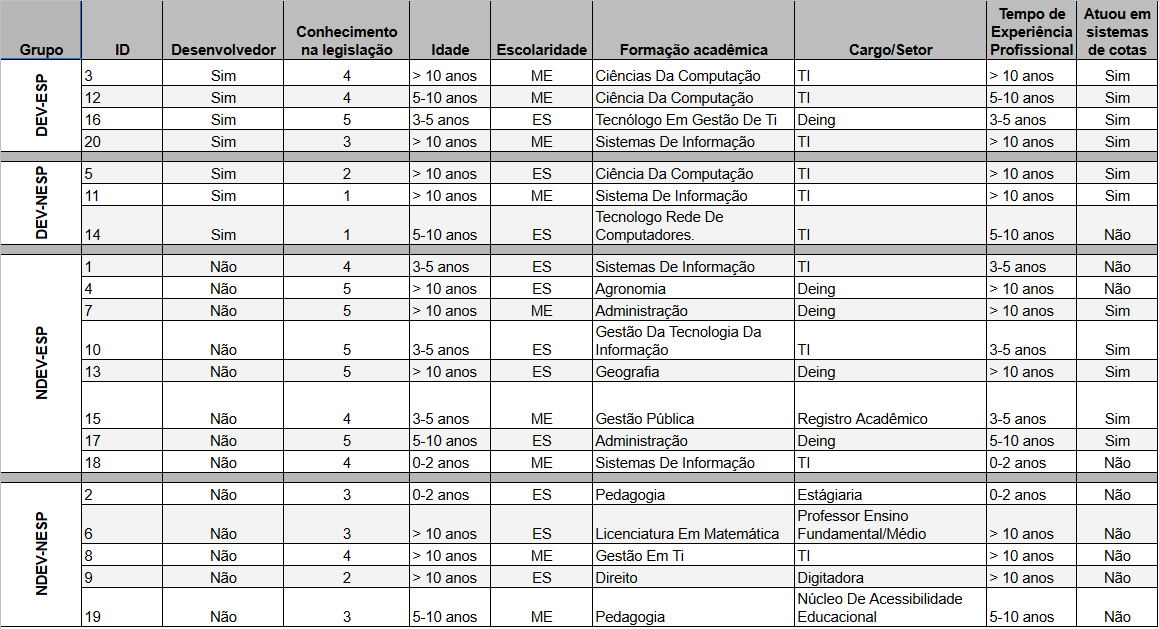
\includegraphics[width=1.5\textwidth]{chapters/analise/imagens/perfilusuarios.png}}

\par\medskip\textbf{Fonte:} Elaboração do autor (2020). \par\medskip

\end{figure}

\end{landscape}

\section{Informações obtidas com o questionário}
\label{sec:perguntasaplicadas}

Esta seção apresenta as perguntas do formulário \textit{on-line} submetido para todos os usuários participantes do presente estudo. As perguntas foram aplicadas após o término da execução do exercício, buscando obter as informações necessárias para cada perfil de usuário da DSL, assim como, entender as principais dificuldades encontradas por eles na utilização da linguagem.

As 5 (cinco) primeiras perguntas tem como objetivo levantar dados demográficos, tais como: nível de formação escolar, curso de formação acadêmica, cargo, tempo de experiência profissional e a informação se elas possuem experiência com desenvolvimento de sistemas.

O formulário \textit{on-line} recebeu 20 respostas, das quais contou com a representatividade de profissionais da área de tecnologia da informação (50\%) e profissionais atuantes em setor de ingresso de estudantes (20\%), além de outros setores como pode ser observado no gráfico da Figura \ref{fig:experienciacargo}. Desses profissionais, 68,4\% indicaram não ter experiência prévia com desenvolvimento de sistemas, enquanto, 31,6\% informaram já terem experiência de desenvolvimento.

\begin{figure}[ht!]
\centering

\caption{\textmd{Cargo e experiência de desenvolvimento}}
\label{fig:experienciacargo}
\fcolorbox{gray}{white}{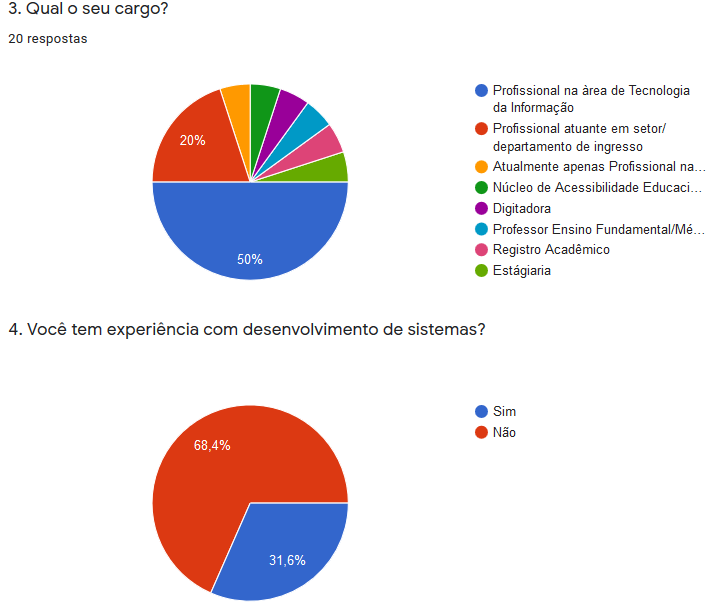
\includegraphics[width=0.80\textwidth]{chapters/analise/imagens/experienciacargo.png}}

\par\medskip\textbf{Fonte:} Elaborada pelo autor (2020). \par\medskip

\end{figure}



\newpage
Para levantar o conhecimento e a experiência sobre o sistema de cotas da rede de ensino federal foram submetidas as seguintes perguntas: "6. Você já atuou em sistemas ou processos seletivos que utilizam regras de classificação para candidatos cotistas?" e "7. Qual o seu grau de conhecimento sobre o sistema de cotas da Lei nº 12.711/2012 e suas atualizações?" (Figura \ref{fig:grauconhecimento}).

\begin{figure}[ht!]
\centering

\caption{\textmd{Perfil de conhecimento e atuação em processos}}
\label{fig:grauconhecimento}
\fcolorbox{gray}{white}{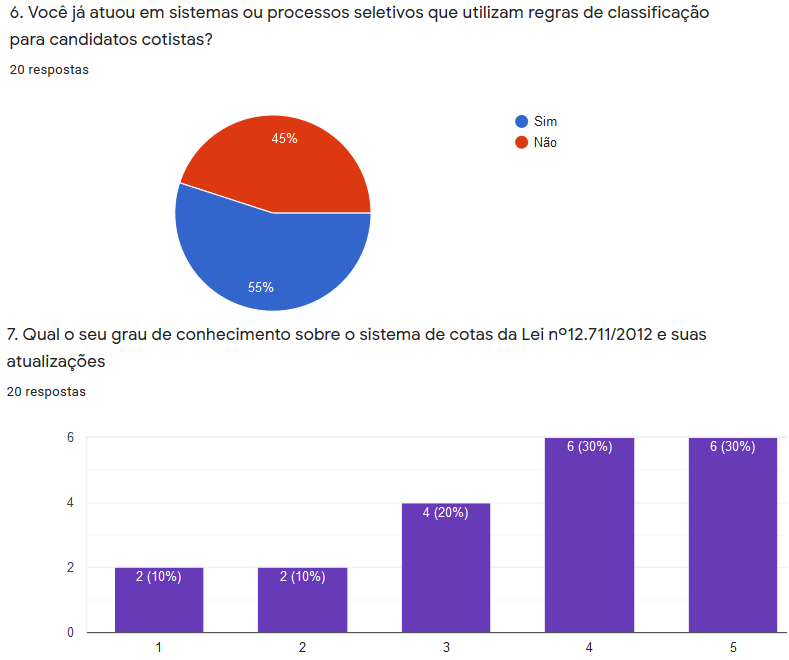
\includegraphics[width=0.85\textwidth]{chapters/analise/imagens/grauconhecimento.png}}

\par\medskip\textbf{Fonte:} Elaborada pelo autor (2020). \par\medskip

\end{figure}



Com o intuito de identificar se os usuários já tiveram contato com outras DSLs, a pergunta "8. Você já utilizou alguma Linguagem de Domínio Específica? Exemplos: HTML, Excel, Latex, SQL, etc.", mostrou que 55\% dos usuários já tiveram contato com outras aplicações ou softwares que utilizam alguma \gls{DSL}, enquanto os demais apontaram não conhecer nenhuma DSL (Figura \ref{fig:usodsl}).

\begin{figure}[ht!]
\centering

\caption{\textmd{Experiência prévia com DSLs}}
\label{fig:usodsl}
\fcolorbox{gray}{white}{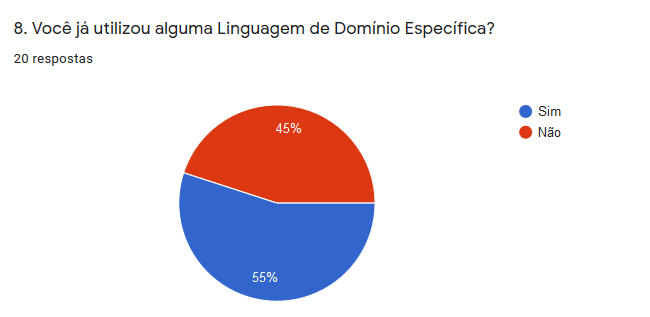
\includegraphics[width=\textwidth]{chapters/analise/imagens/usodsl.png}}

\par\medskip\textbf{Fonte:} Elaborada pelo autor (2020). \par\medskip

\end{figure}



\newpage
Em continuidade, foram adicionadas as seguintes perguntas responsáveis pelo levantamento de dificuldades de uso com a DSL:

\begin{enumerate}

    \item[a)] 9. De modo geral, qual o grau de dificuldade para execução do exercício proposto?;
    
    \item[b)] 10. Considerando a sua resposta na pergunta anterior, qual(is) a(s) dificuldade(s) encontrada(s)?;
    
    \item[c)] 11. Na sua avaliação quais as principais limitações da linguagem proposta?  ;
    
   \item[d)]  12. Quais dos materiais abaixo você utilizou para execução do exercício?;
   
   \item[e)] 13. No caso de a linguagem apresentar erros "destaques em vermelho" ou avisos "destaques em amarelo", as mensagens foram claras e ajudaram a resolver o(s) problema(s) apresentado(s)?;
   
   \item[f)] 14. Quanto tempo, aproximadamente, você utilizou para executar o exercício proposto?.   

\end{enumerate}

Em linhas gerais, o grau de dificuldade de uso da DSL, em escala de 1 (difícil) e 5 (fácil), pode ser observado na Figura \ref{fig:dificuldadegeral}. O formulário completo foi disponibilizado no (APÊNDICE \ref{chap:apen:formularioapen}). 

\begin{figure}[ht!]
\centering

\caption{\textmd{Dificuldade de uso e deficiências da DSL}}
\label{fig:dificuldadegeral}
\fcolorbox{gray}{white}{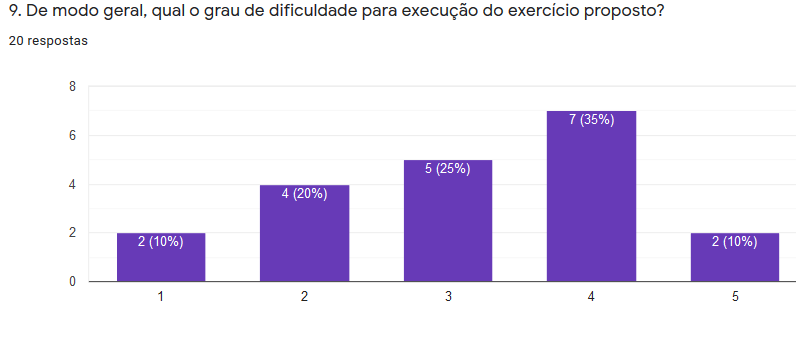
\includegraphics[width=0.85\textwidth]{chapters/analise/imagens/dificuldadegeral.png}}

\par\medskip\textbf{Fonte:} Elaborada pelo autor (2020). \par\medskip

\end{figure}



\newpage
Os demais resultados obtidos com o formulário e os exercícios são descritos com maiores detalhes nas próximas Seções.




\section{Resultados obtidos com o exercício}
\label{sec:analiseexercicio}

Cada usuário recebeu por e-mail um manual  contendo as principais instruções para uso da DSL Cotas, incluindo conceitos sobre cada elemento da legislação. Adicionalmente, a esse manual foi definido um exercício aberto, no qual, a tarefa proposta é definir os requisitos da primeira versão da lei nº 12.711 (Figura \ref{fig:exercicio}). 

\begin{figure}[ht!]
\centering

\caption{\textmd{Versão proposta para exercício da DSL}}
\label{fig:exercicio}
\fcolorbox{gray}{white}{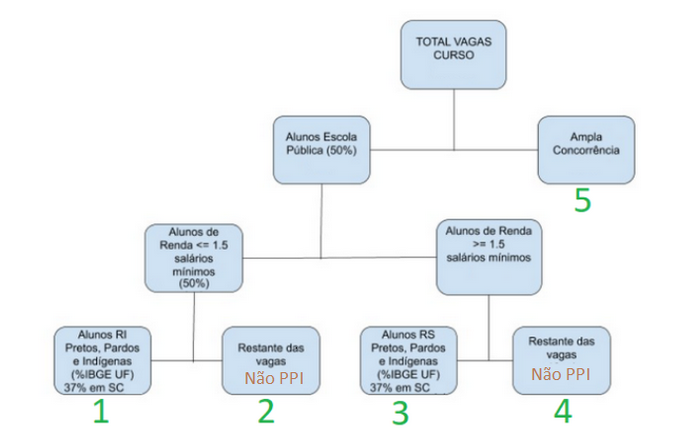
\includegraphics[width=0.85\textwidth]{chapters/analise/imagens/exercicio.png}}

\par\medskip\textbf{Fonte:} Elaboração do autor (2020). \par\medskip

\end{figure}



Essa versão foi escolhida por ser mais simples se comparada as versões mais recentes, requerendo um tempo menor de dedicação ao exercício e adequando a complexidade para todos os grupos dos diferentes perfis de usuários. 


Com o intuito de avaliar o exercício, todas as 20 respostas foram salvas imediatamente após o término no sistema de controle de versão \texttt{git}. Cada resposta foi salva em um \texttt{branch} disponível no repositório \texttt{https://github.com/spgroup/dsl-cotas/branches}.


Durante essa análise foram contabilizados os acertos em relação aos seguintes elementos da linguagem: distribuição de vagas (níveis e categorias criadas), configurações de percentuais (definição e utilização durante a distribuição), definição completa da ordem de prioridade (ordem indicada e quantidade de categorias presentes), quantidade de \textit{errors} e \textit{warnings} não resolvidos, e a presença de versão da legislação mais recente implementada opcionalmente por alguns usuários.

A seguir são apresentados os resultados da aplicação do exercício para cada grupo.


\subsection{Resultados do Grupo DEV-ESP}
\label{subsec:devesp}

Em relação à pergunta "9. De modo geral, qual o grau de dificuldade para execução do exercício proposto?", em uma escala de 0(difícil) e 5(fácil), nesse grupo de usuários todos indicaram a nota 4 e 5. Ademais, foram realizadas as seguintes considerações:

\begin{enumerate}
    \item [a)] "Dúvidas de primeiro uso, do tipo -o que  mesmo que eu devia digitar maiúsculo?-, -será que preciso mesmo digitar 50.0 ou só 50?-,  entre outras do gênero. Como é execução de um exercício que é feito pela primeira vez, esse tipo de dúvida acaba não deixando totalmente fácil, pois eventualmente é necessário rever alguma instrução. Mas de resto, se já tiver esses detalhes na cabeça, a execução seria bem fácil (Usuário 20).";
    
    \item[b)] "A sequência de prioridades final onde se define quais candidatos se seleciona primeiro, foi um pouco mais difícil fazer a seleção... A dificuldade do último item pode ser melhorada com implementação ou instruções. No mais ficou bem interessante para configurar a árvore de decisão e percentuais aplicados (Usuário 3).".
\end{enumerate}

Conforme relatado pelo Usuário 20, no primeiro contato com a DSL surgem algumas dúvidas sobre o formato de preenchimento dos percentuais e de siglas de categorias, o que pode levar a necessidade de reescrita de algumas instruções da linguagem. De modo geral, isso pode ser resolvido a medida que se acostuma com a linguagem.

Outro aspecto levantado pelo Usuário 3 relaciona-se com problemas durante a definição da ordem de prioridade, em que o comando de adição de novos itens na lista não estava claro o suficiente na linguagem, sendo necessário melhorar a usabilidade desse elemento.

Os exercícios foram finalizados entre 15 a 30 minutos, sendo que 2 (dois) desses usuários (Usuário 20 e 16) fizeram completamente a definição da árvore de distribuição, sem \textit{errors} ou \textit{warnings}. Os outros dois usuários (Usuário 3 e 12) não resolveram alguns erros e avisos da linguagem, um deles criou um nível a mais de distribuição, gerando uma árvore de distribuição incorreta (Figura \ref{fig:errodevesp}). 

\begin{figure}[ht!]
\centering

\caption{\textmd{Exercício com erro na árvore de distribuição}}
\label{fig:errodevesp}
\fcolorbox{gray}{white}{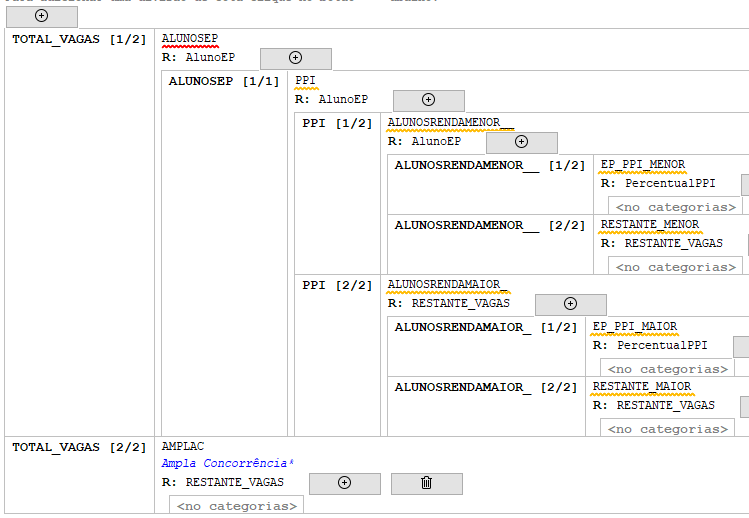
\includegraphics[width=0.85\textwidth]{chapters/analise/imagens/figerrodevesp.png}}

\par\medskip\textbf{Fonte:} Dados da pesquisa (2020). \par\medskip

\end{figure}






Com relação às respostas presentes na questão "11. Na sua avaliação quais as principais limitações da linguagem proposta?", 2 (dois) usuários informaram que: "As sugestões das mensagens informativas não são claras o suficiente (Usuários 16 e 20)", o que pode ter levado aos problemas descritos anteriormente.

Em relação a pergunta "13. No caso de a linguagem apresentar erros "destaques em vermelho" ou avisos "destaques em amarelo", as mensagens foram claras e ajudaram a resolver o(s) problema(s) apresentado(s)?", esse grupo indicou conseguir de maneira geral resolver os problemas tendo como base as mensagens apresentadas pela DSL, todos indicaram a pontuação de escala 4 e 5 (quatro e cinco), considerando a escala de 1(difícil) e 5(fácil).

Contudo, após o levantamento apresentado na Figura \ref{fig:quadro:grupodevesp}, foi possível identificar que os demais recursos e percentuais foram preenchidos corretamente. Destaca-se que o grupo em análise, possui bom conhecimento na área de domínio, além de ter familiaridade com ferramentas de desenvolvimento e outras \gls{DSL}s, o que pode ter sido preponderante para que tenham indicado que a linguagem foi de fácil uso e entendimento. 
\begin{figure}[ht!]
\centering

\caption{\textmd{Quadro da análise do grupo DEV-ESP}}
\label{fig:quadro:grupodevesp}
\fcolorbox{gray}{white}{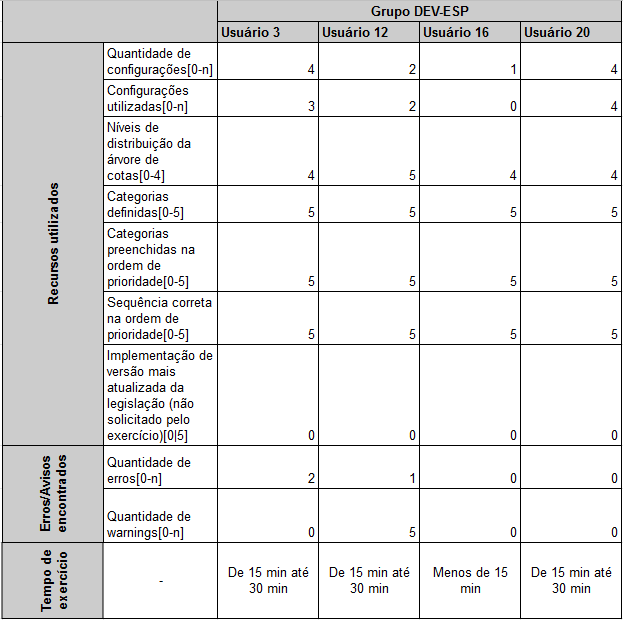
\includegraphics[width=0.85\textwidth]{chapters/analise/imagens/grupodevesp.png}}

\par\medskip\textbf{Fonte:} Elaboração do autor (2020). \par\medskip

\end{figure}


\newpage
\subsection{Resultados do Grupo DEV-NESP}
\label{subsec:devnesp}

Nesse grupo, com relação à pergunta sobre o grau de dificuldade, os usuários apontaram os níveis 2 e 3 (três e dois), considerando a escala de 1(difícil) e 5(fácil). No exercício do Usuário 6 constaram vários erros não resolvidos na distribuição de vagas, em sua maioria em relação ao padrão de nomenclatura das siglas das categorias de cotas (Figura \ref{fig:errodevnesp}). 

\begin{figure}[ht!]
\centering

\caption{\textmd{Exercício do Usuário 11}}
\label{fig:errodevnesp}
\fcolorbox{gray}{white}{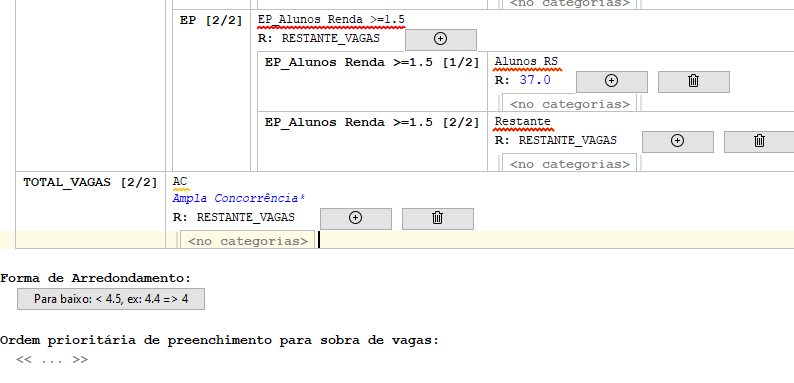
\includegraphics[width=0.85\textwidth]{chapters/analise/imagens/figerrodevnesp.png}}

\par\medskip\textbf{Fonte:} Elaboração do autor (2020). \par\medskip

\end{figure}



\newpage


Adicionalmente à questão sobre o grau de dificuldade foram feitos os seguintes comentários:

\begin{enumerate}
    \item [a)] "Foi difícil entender o funcionamento do sistema (Usuário 5)";
    \item [b)] "No exercício não compreendi se era pra utilizar a a ordem de prioridade ou não, se segue o padrão de uma árvore ou teria que informar. A questão do arredondamento ficou um pouco confusa, depois que entendi que é apenas uma configuração caso utilizar números quebrados nos percentuais (Usuário 11)";
    \item [c)] "Tive dificuldade em entender a proposta por não conhecer a lei específica.  (Usuário 14)".    
\end{enumerate}

Portanto, nota-se a dificuldade de entendimento de questões relacionadas à legislação do sistema de cotas e, adicionalmente, algumas dificuldades sobre uso do elemento de ordem de prioridade da linguagem. 

Em continuidade a essa análise, apresentam-se as considerações para a pergunta que trata sobre as limitações da linguagem: "Não observei a execução de uma emulação de processo em prática (Usuário 5)", "As sugestões das mensagens informativas não são claras o suficiente (Usuário 11)".

Considerando a limitação apontada pelo Usuário 5, observa-se a falta do \textit{feedback} por parte da DSL para simulação da distribuição de vagas, uma vez que a função responsável por fazer os cálculos do quadro de vagas foi implementada apenas na API DSL Cotas. 

Novamente foram apontados problemas nas mensagens geradas pela linguagem, conforme relato do Usuário 11. Esse usuário afirma que: "O vídeo didático poderia ser mais alto e com mais instruções de utilização.", indicando que são necessárias mais instruções no manual e no vídeo explicativo para conseguir melhorar o entendimento da linguagem. 

Ademais, as seguintes sugestões foram levantadas por meio da pergunta número 15 do questionário:

\begin{citacao}
A linguagem auxilia a documentar o processo. Acredito que ela implemente a execução da coleta de dados. Espero que ela saiba ler os dados de várias bases diferentes, e não exija um tratamento nestes dados muito extenso, senão é talvez mais viável inserir diretamente os dados em uma base relacional e executar as ordenações necessárias (Usuário 5).
\end{citacao}

Tendo em vista os apontamentos descritos para o grupo, observa-se que a falta de entendimento nas regras de domínio dificulta o uso da linguagem (Usuários 11 e 14), no entanto, há maiores preocupações relacionadas à simulação e aos detalhes de implementação para o processamento final das regras (Usuário 5). Conforme o levantamento descrito na Figura \ref{fig:quadro:grupodevnesp},  observou-se um tempo maior para o exercício do Usuário 5 (Mais de 30min).

\begin{figure}[ht!]
\centering

\caption{\textmd{Quadro da análise do grupo DEV-NESP}}
\label{fig:quadro:grupodevnesp}
\fcolorbox{gray}{white}{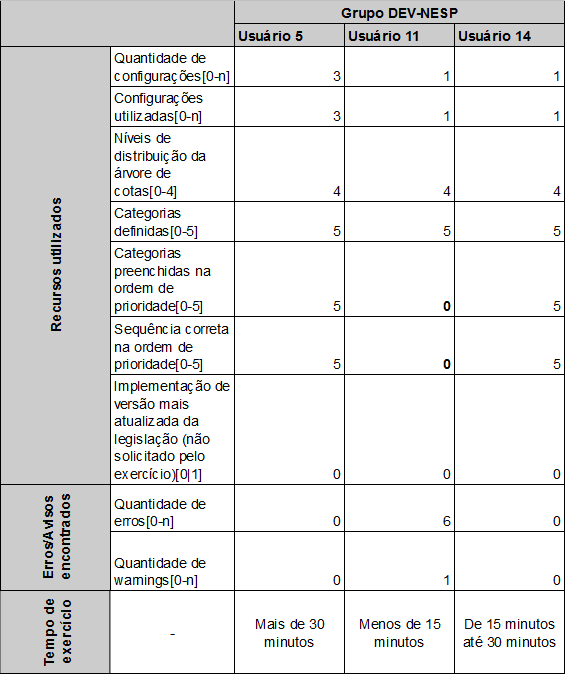
\includegraphics[width=0.77\textwidth]{chapters/analise/imagens/grupodevnesp.png}}

\par\medskip\textbf{Fonte:} Elaborada pelo autor (2020). \par\medskip

\end{figure}






\newpage
\subsection{Resultados do Grupo NDEV-ESP}
\label{subsec:ndevesp}

Nessa Subseção são analisados os dados dos participantes cujos perfis indicam maior proximidade com os usuários finais da DSL Cotas. Esses usuários, em sua maioria, já participaram da organização de processos seletivos com base no sistema de cotas, no entanto, não possuem nenhuma experiência com ferramentas de desenvolvimento de sistemas.

A Figura \ref{fig:dificuldadendevesp} demonstra o gráfico elaborado para as 8 (oito) respostas do grupo em relação à pergunta 11 do formulário, na qual em uma escala de 1 (difícil) a 5 (fácil) foi possível identificar que 50\% dos usuários tiveram maior facilidade (escala 4), 25\% indicaram a escala intermediária de dificuldade (escala 3) e os demais consideraram o uso da DSL como difícil (escalas 1 e 2). 

\begin{figure}[ht!]
\centering

\caption{\textmd{Gráfico de respostas com a escala de dificuldade}}
\label{fig:dificuldadendevesp}
\fcolorbox{gray}{white}{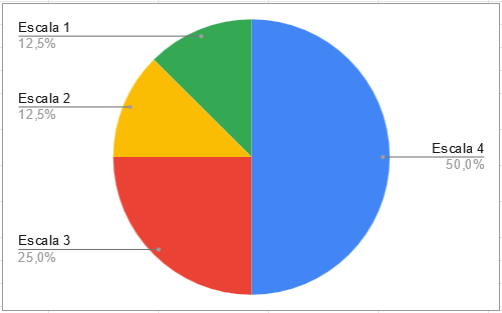
\includegraphics[width=0.85\textwidth]{chapters/analise/imagens/dificuldadendevesp.png}}

\par\medskip\textbf{Fonte:} Elaborado pelo autor (2020). \par\medskip

\end{figure}



Considerando os comentários dos usuários sobre essa pergunta, destacam-se as seguintes observações:

\begin{enumerate}
    \item [a)] "É necessário familiarizar-se com o ambiente proposto para o exercício.  (Usuário 1)";
    
    \item [b)] "Apenas dificuldade inicial para entender a lógica dos comandos. Logo após este entendimento, tornou-se fácil a utilização. O tutorial está muito claro, mas talvez um melhor suporte com menagens informativas no próprio ambiente, ao clicar nas etapas (Usuário 7)";
    
    \item [c)] "Primeiro momento parece simples, mas como preencher corretamente, as siglas finais, fiquei um pouco confusa, e ao preencher um percentual no próximo só dar ctrl + backspace ou somente colocar RESTANTE\_VAGAS... No final da ordem de como vai ser preenchido os restantes de vaga precisava ser um pouco mais claro, .. no geral é uma ótima ferramenta, mas necessitaria mais algumas aulas para ficar fera (Usuário 10)";
    
    \item [d)] "Demorei um pouco para entender o funcionamento, a regra do sistema, mesmo após ver o vídeo explicativo. Após isso, interpretar a lei, ou o exercício, e aplicar no sistema também surtiu uma certa dificuldade - refiz 3 vezes até entender que estava de acordo com o proposto (Usuário 13)";
    
    \item[e)] "O preenchimento na distribuição de vagas, sendo o entendimento do funcionamento das regras, após ter uma dificuldade com a variável pré existente de RESTANTE\_VAGAS, e a relação com as configurações acima, o procedimento ficou mais claro (Usuário 18)".
\end{enumerate}

Portanto, observa-se que esse grupo teve dificuldades relacionadas ao uso de comandos e regras da DSL, no que concerne à etapa de distribuição de vagas. Todos os usuários citados relatam que essas dificuldades foram resolvidas após algum tempo de uso da DSL Cotas.

Destaca-se que, 2 (dois) usuários do grupo (Usuário 4 e 7), implementaram a versão mais atualizada da legislação, na qual é composta de 5(cinco) níveis de distribuição e 9 (nove) categorias, incluindo a subdivisão para candidatos PCD (Figura \ref{fig:ndevesp}). Essa versão não foi proposta pelo exercício e, mesmo assim, esses usuários avançaram na utilização da DSL Cotas opcionalmente. Isso pode indicar que, apesar das dificuldades encontradas, foi possível utilizar a DSL Cotas até para situações mais complexas não previstas pelo exercício.


\begin{figure}[ht!]
\centering

\caption{\textmd{Exercício com a versão atualizada da lei}}
\label{fig:ndevesp}
\fcolorbox{gray}{white}{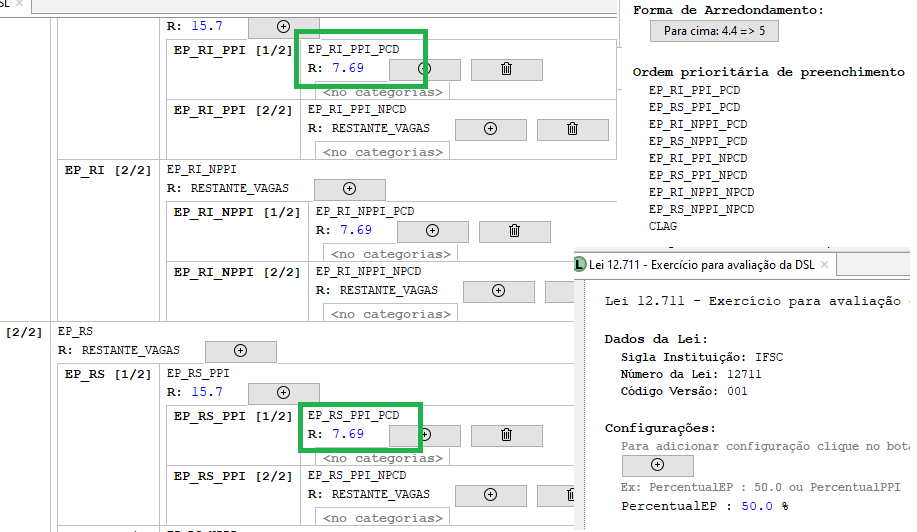
\includegraphics[width=\textwidth]{chapters/analise/imagens/figndevesp.png}}

\par\medskip\textbf{Fonte:} Dados da pesquisa (2020). \par\medskip

\end{figure}



Nesse grupo, o Usuário 4 levou mais de 1 (uma) hora para fazer a implementação do exercício, embora este também tenha utilizado a versão mais recente como base para descrição na DSL Cotas. Os demais, em sua maioria, conseguiram finalizar o exercício entre 15 e 30 minutos (Figura \ref{fig:quadro:grupondevesp}).

\begin{figure}[ht!]
\centering

\caption{\textmd{Quadro da análise do grupo NDEV-ESP}}
\label{fig:quadro:grupondevesp}
\fcolorbox{gray}{white}{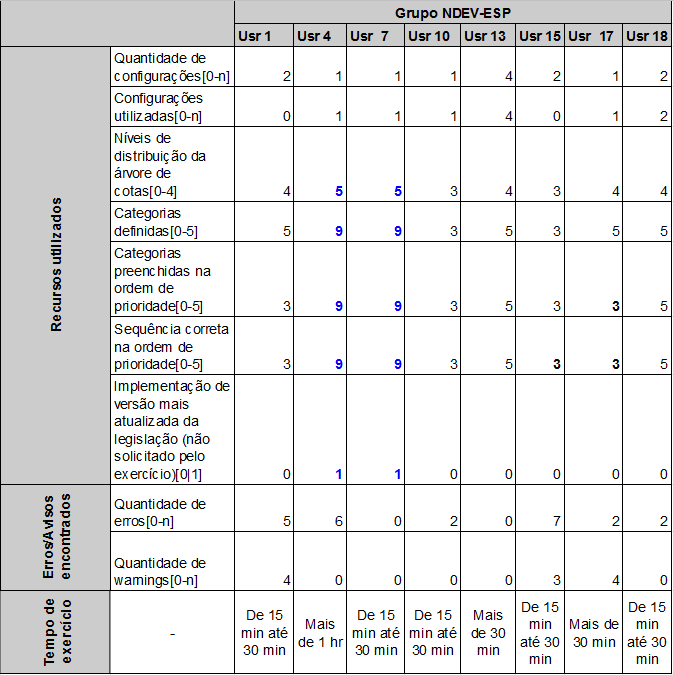
\includegraphics[width=0.85\textwidth]{chapters/analise/imagens/grupondevesp.png}}

\par\medskip\textbf{Fonte:} Elaboração do autor (2020). \par\medskip

\end{figure}



Sobre a pergunta "11. Na sua avaliação quais as principais limitações da linguagem proposta?", 4 (quatro) usuários apontaram que a principal limitação é: "As sugestões das mensagens informativas não são claras o suficiente". O Usuário 13 relatou que "O layout talvez não seja tão amigável para leigos em programação, o que dificulta um pouco para identificar onde clicar e o que digitar".

Assim como nos demais grupos de usuários, o grupo NDEV-ESP sugere melhorias nas mensagens informativas e na apresentação dos elementos da linguagem. Adicionalmente, algumas considerações foram observadas após análise do questionamento número "15. Comentários e Sugestões":

\begin{enumerate}
    \item [a)] "A fim de evitar erros e facilitar a compreensão, o sistema poderia apresentar, ao operador, uma simulação da distribuição de vagas para cada cota. Ex: Inicialmente o sistema mostra na variável RESTANTE\_VAGAS o valor 100 (ou outro valor). Após inserida a cota de ampla concorrência (CLAG) com percentagem de 50\%, a variável RESTANTE\_VAGAS apresenta o valor 50 e a CLAG apresenta o valor 50. E assim para todas as outras cotas. Ao final, seriam apresentadas as quantitativos de vagas para cada uma das cotas conforme os quadros dos editais de ingresso. (Usuário 1)";
    \item [b)] "O ambiente parece bastante prático e dinâmico, com facilidade de adaptação às necessidades de cada tipo de processo seletivo. (Usuário 7)";    
    \item [c)] "O manual de instruções está bem explicado, porém, por ser uma linguagem nova, pode haver dificuldade na interpretação das instruções, como foi meu caso. Confundi algumas instruções simples pois fiquei focado tentando entender os demais comandos que não conhecia. Porém, saliento que após utilizar a primeira vez, o sistema é de fácil manuseio. (Usuário 17)";   
    \item [d)] "Não tem um entendimento claro sobre as configurações de percentual. Ex: quando nas configurações eu preencho um percentual de PPI -  este é sobre o valor total ou sobre o valor da categoria que ele pertencer posteriormente. (Usuário 18)".
\end{enumerate}

Esses comentários rementem às sugestões de melhorias, tais como: a necessidade de simulação prévia da distribuição e maior clareza sobre o modo de configuração dos percentuais das categorias. Ademais, apesar de dificuldades na interpretação e uso dos comandos (Usuário 17), observou-se que há facilidade de adaptação às necessidades de cada tipo de processo seletivo (Usuário 7).

Por fim, considerando que os usuários do grupo conseguiram avançar no uso da DSL Cotas já no primeiro contato com a linguagem, mesmo sem ter conhecimento em desenvolvimento de sistemas, conclui-se que após terem maior familiaridade com a ferramenta, os usuários com domínio nas regras do sistema de cotas conseguem utilizar a DSL como meio de descrever as regras existentes na legislação.


\subsection{Resultados do Grupo NDEV-NESP}
\label{subsec:ndevnesp}

Diferentemente dos grupos de usuários desenvolvedores e especialistas, que são os principais envolvidos no processo de compreensão e implementação da legislação, o grupo NDEV-NESP foi escolhido para verificar se o design da DSL Cotas é simples o suficiente para pessoas leigas no assunto. Com isso, na medida em que sintam necessidade, consigam compreender mais facilmente o funcionamento das regras de cotas com o uso da DSL, seja por interesse próprio ou pelo fato de, por exemplo, precisarem atuar em setores ou ações institucionais que envolvam processos de classificação de candidatos.


Com relação ao levantamento da cursos da formação acadêmica do grupo foram informados os seguintes cursos: Pedagogia, Licenciatura em Matemática, Gestão em TI e Direito. Os dados levantados sobre o cargo atual dos usuários foram: Professor Ensino Fundamental/Médio, Estagiário, TI, Digitador e Profissional do Núcleo de Acessibilidade Educacional.

Em relação ao tempo de execução do exercício, esse grupo apresentou resultado variado. Os Usuários 6 e 19 levaram mais de 30 minutos, os Usuários 2 e 9 levaram de 15 até 30 minutos e o Usuário 8 levou menos de 15 minutos (Figura \ref{fig:quadro:grupondevnesp}). 

\begin{figure}[ht!]
\centering

\caption{\textmd{Quadro da análise do grupo NDEV-NESP}}
\label{fig:quadro:grupondevnesp}
\fcolorbox{gray}{white}{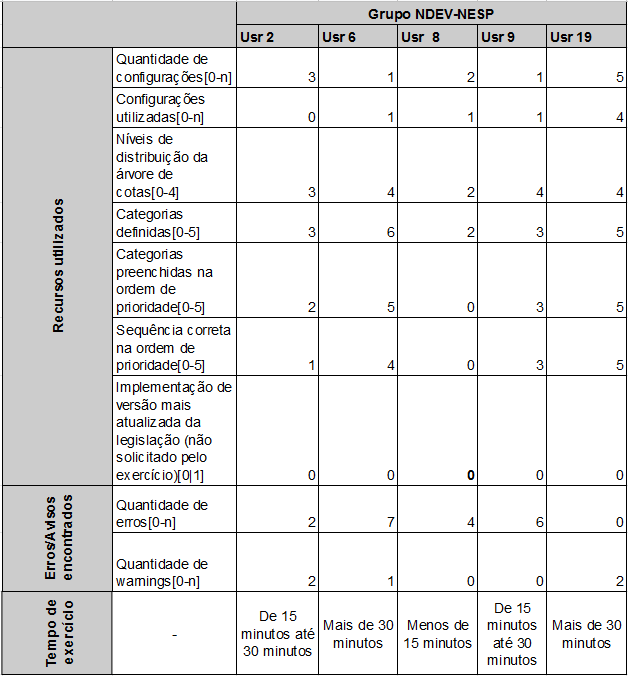
\includegraphics[width=0.80\textwidth]{chapters/analise/imagens/grupondevnesp.png}}

\par\medskip\textbf{Fonte:} Elaboração do autor (2020). \par\medskip

\end{figure}


\newpage

Após o levantamento, foi possível identificar que 3 (três) dos 5 (cinco) usuários, não implementaram corretamente a quantidade de níveis de distribuição proposta pelo exercício, os Usuários 2 e 8 implementaram, respectivamente, apenas 3 (três) e 2 (dois) níveis da árvore. O Usuário 6 criou um nível extra sem subdivisões o que gerou um número de 6 categorias. Os problemas criados durante a definição da distribuição ocasionaram no aumento da contabilização de erros para esse grupo. 

Destaca-se o caso do Usuário 2, o qual utilizou a constante RESTANTE\_VAGAS fora do contexto de distribuição, o que levou o pesquisador a descobrir uma falha durante a checagem de escopo da DSL Cotas (Figura \ref{fig:falha}). Ademais, o Usuário 8 acabou desistindo da correção dos erros apontados pela DSL Cotas no segundo nível de distribuição, indicando a finalização do exercício abaixo de 15 minutos (Figura \ref{fig:figerroniveis}).

\begin{figure}[ht!]
\centering

\caption{\textmd{Falha nas restrições de escopo}}
\label{fig:falha}
\fcolorbox{gray}{white}{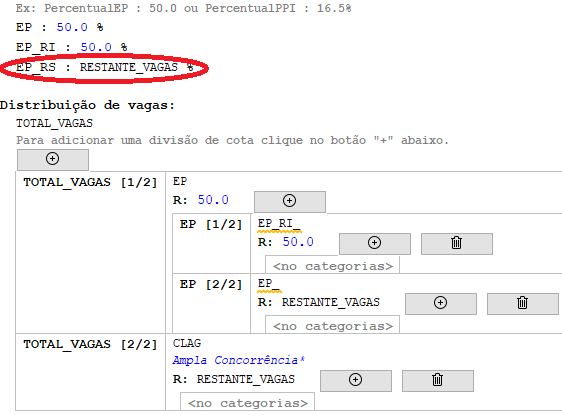
\includegraphics[width=\textwidth]{chapters/analise/imagens/figfalha.png}}

\par\medskip\textbf{Fonte:} Dados da pesquisa (2020). \par\medskip

\end{figure}



\begin{figure}[ht!]
\centering

\caption{\textmd{Problemas na definição da distribuição}}
\label{fig:figerroniveis}
\fcolorbox{gray}{white}{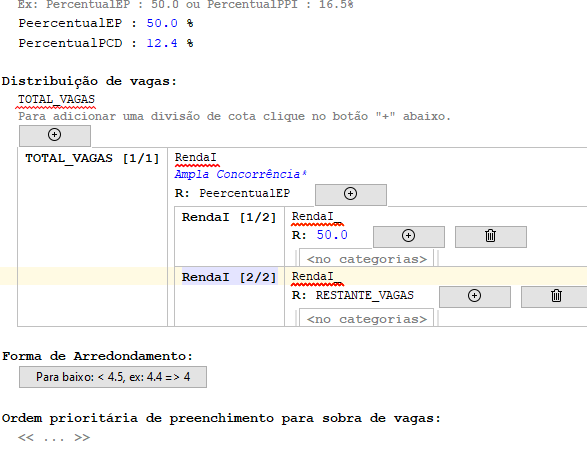
\includegraphics[width=0.85\textwidth]{chapters/analise/imagens/figerroniveis.png}}

\par\medskip\textbf{Fonte:} Dados da pesquisa (2020). \par\medskip

\end{figure}



\newpage
Para o levantamento sobre o grau de dificuldade nas escalas 1 (difícil) até 5 (fácil) observa-se que os Usuários: 2, 6 e 19 apontaram a escala 3, enquanto os usuários 8 e 9 apontaram a escala 4 e 2, respectivamente. O que pode indicar que na maioria dos casos houve dificuldade para entendimento e uso da DSL Cotas.

Em continuidade à análise das dificuldades, consideram-se as seguintes observações dos usuários:

\begin{enumerate}
    \item [a)] "Uma das dificuldades é por ser o primeiro contato com a ferramenta e não ter domínio sobre a mesma. Depois, fiquei com dúvida no preenchimento dos critérios: Eles serão baseados na lei de cotas, ou seja, os percentuais de destinação para cada vaga já estão estabelecidos, fica a critério de quem for criar a árvore a ordem de destino das vagas então? Fiquei com dúvida também se as abreviações deveriam ser conforme o que já consta nos editais e como os inscritos se cadastram no sistema de ingresso, ou se isso não faz diferença. (Usuário 2)"; 
    \item [b)] "Como usuário iniciante, o guia de instruções estava com poucas informações para execução da tarefa. (Usuário 6)";     
    \item [c)] "Como pessoa que não exerce atividade nesse segmento, achei pouco intuitivo. A parte para definição de ordem prioritária, aparentava existirem campos repetidos, pois referente aos alunos RI e RS não encontrei diferenciação entre os 37\% e o restante de vagas (dá a ideia de existirem apenas 3 campos - Alunos RI - Alunos RS - AC). (Usuário 9)";
    \item [d)] "Para organizar as informações no exercício precisei rever o vídeo com as instruções e após a segunda visualização do material com exemplos consegui usar os recursos mais facilmente. (Usuário 19)".     
\end{enumerate}

Desse modo, pontuam-se algumas das dificuldades apresentadas por esse grupo, tais como: dúvidas sobre o preenchimento correto dos percentuais e siglas das categorias (Usuário 2), falta de instruções com passos mais detalhados (Usuário 6), problemas durante a definição das categorias e sua utilização na ordem de prioridade (Usuário 9) e a necessidade de várias consultas no manual e ao vídeo explicativo da DSL (Usuário 19). 

Com relação ao levantamento sobre as deficiências da linguagem, os Usuários 2 e 19 marcaram a opção "O tempo de aprendizagem da linguagem é extenso", enquanto os demais usuários apontaram que "As sugestões das mensagens informativas não são claras o suficiente". 

Em sequência a esse levantamento, os usuários apontaram como comentários e sugestões: 

\begin{enumerate}
    \item [a)] "Achei o sistema em certa medida intuitivo e de fácil manuseio, mas tive dificuldades com o tamanho da fonte das palavras (estava pequeno e não foi possível aumentar usando ctrl+). Acredito que com critérios bem estabelecidos (quais abreviações usar, etc) e um tempo maior de uso a ferramenta será de grande utilidade (Usuário 2)";
    \item[b)] "O guia para 1ª utilização do sistema poderia ser mais detalhado; mensagens de erro poderiam ser exibidas em caixas de texto; tamanho das letras nas caixas de opções, muito pequenas. (Usuário 6)";
    \item[c)] "Nas mensagens de erro ou aviso, constar exemplo correto de preenchimento. (Usuário 8)".   
\end{enumerate}

Por fim, notou-se maior dificuldade de entendimento das mensagens e nos recursos de \textit{feedback} ao usuário, se comparado aos grupos com conhecimento na área de domínio e/ou desenvolvimento de sistemas. Na Subseção \ref{sec:comparativogrupos} é descrito o resumo comparativo entre os grupos analisados.

\subsection{Comparativo entre os grupos de análise}
\label{sec:comparativogrupos}

Em relação aos critérios estabelecidos para a análise, considerando o levantamento apresentado pelas Figuras \ref{fig:quadro:grupodevesp}, \ref{fig:quadro:grupodevnesp}, \ref{fig:quadro:grupondevesp} e \ref{fig:quadro:grupondevnesp}, observou-se que o grupo DEV-ESP teve mais facilidade de entendimento e utilização dos recursos da DSL, uma vez que todos os usuários conseguiram definir as regras propostas pelo exercício, além das soluções apresentarem poucos \textit{errors} e \textit{warnings}. Esse fato reforça que: "o uso de DSLs com entendimento do domínio, deixa o pensamento ser expresso de maneira mais clara quando o código escrito não está repleto de detalhes de implementação"  \cite[p.41, tradução nossa]{dslengineering}.

Em segundo lugar, considerando a correta implementação das regras propostas, no grupo NDEV-ESP apenas 2 (dois) dos 8 (oito) usuários não conseguiram configurar a distribuição completa, no entanto, 6 (seis) usuários fizeram as definições conforme o exercício, sendo que 2 (dois) deles avançaram no desenvolvimento da versão mais recente e complexa da legislação, contemplando candidatos inscritos na categoria PCD. 

O fato dos usuários NDEV-ESP terem conseguido atender uma legislação diferente da proposta, pode se relacionar com um dos benefícios de DSLs: 

\begin{citacao}
O uso de DSLs específicas de domínio, podem parecer, a primeiro momento, difícil de se justificar, porém essas DSLs são normalmente atreladas ao \textit{know-how} do negócio, provendo um meio de descrever conhecimento de maneira formal, organizada e sustentável. \cite[p.43, tradução nossa]{dslengineering}.
\end{citacao}

Em continuidade a esse comparativo, o grupo DEV-NESP ficou em terceiro lugar no que diz respeito ao entendimento sobre os recursos utilizados, esses usuários apontaram no questionário um grau de dificuldade elevado, o que foi agravado pelo fato de desconhecerem a área de domínio. Contudo, apesar das dificuldades, na maioria dos casos, todos os recursos foram utilizados sem que fossem gerados muitos erros ou avisos. 

Por fim, a análise do grupo NDEV-NESP mostra que há potencial de uso da DSL, no entanto, destaca-se que há necessidade de mais explicações sobre as regras de domínio, assim como de capacitação para uso na linguagem. Isso se justifica, pelo fato de que esse grupo apresentou maior quantidade de erros além de alguns exercícios terem sido entregues de forma incompleta.



\subsection{Mudanças resultantes da avaliação}
\label{sec:mudanasresultantes}

Considerando as principais dificuldades relatadas pelos usuários da DSL Cotas, nessa Subseção são descritas as melhorias implementadas na linguagem que foram selecionadas com o objetivo de reduzir as lacunas de entendimento sobre a distribuição das vagas e também melhorar a clareza das mensagens de erros e avisos aos usuários.

A primeira melhoria é a responsável pelo tratamento das sugestões apontados pelos usuários do grupo DEV-ESP e NDEV-ESP, os quais apontaram a necessidade de visualização prévia de simulação das vagas, para tanto foi adicionado um novo elemento do tipo \texttt{behavior}, \texttt{Distribuicao\_Behavior} no qual foram inseridos métodos para varrer a \gls{AST} e fazer os cálculos do quadro de vagas seguindo as definições preenchidas pelo usuário da DSL (Código Fonte \ref{lst:distribuicao_behavior}).

\newpage

\lstinputlisting[language=Java, 
caption=Behavior para cálculo do quadro de vagas 
,label=lst:distribuicao_behavior]{chapters/trechos_codigo/distribuicao_behavior.m}


O método \texttt{calculaDistribuicao} (Linha 3) acessa a \texttt{CategoriaCota} raiz, o valor de simulação desejado e a forma de arredondamento definida pelo usuário, e em sequência, por meio do método recursivo \texttt{calculaVagasCategoria} (Linha 14) são realizadas iterações em todas as categorias subsequentes da distribuição, calculando as vagas conforme os respectivos percentuais (Linha 24) ou fazendo o cálculo de soma das vagas para a constante \texttt{RESTANTE\_VAGAS} (Linha 27). 

Os números de vagas para cada categoria são armazenados em um novo atributo do conceito, nomeado de \texttt{numeroVagas}, esses valores são atualizados sempre que o usuário aciona a função de simulação na DSL ou no caso da forma de arredondamento ser alterada. Desse modo foi possível adicionar novos elementos no editor dos conceitos \texttt{CategoriaCota} e \texttt{Distribuicao} para apresentar o valor calculado, além de gerar uma listagem do quadro de vagas (Figuras \ref{fig:editoralterado}, \ref{fig:simulacaovagas} e \ref{fig:quadrosimulacao}).


\input{chapters/analise/imagens/editoralterado}

\clearpage
\input{chapters/analise/imagens/quadrosimulacao}


A visualização prévia dos cálculos pode auxiliar no entendimento dos requisitos de distribuição de vagas para todos os grupos de usuários analisados, possibilitando que tenham uma simulação imediata dos elementos da linguagem, além de auxiliar no caso de dúvidas sobre como os percentuais são aplicados no contexto da árvore de distribuição.

Com relação às dificuldades de entendimento das mensagens de erro e dos avisos apresentados pela linguagem, foram alteradas as instruções para incluir exemplos de formato de preenchimento, além de tratamentos para priorizar as mensagens exibidas de modo que não fossem geradas inconsistências antecipadamente, o que pode contribuir para confundir o usuário sobre o momento correto da sua resolução (Figura \ref{fig:mensagens}).

\input{chapters/analise/imagens/mensagens}

No que diz respeito às dificuldades dos usuários para seleção das categorias na seção \texttt{OrdemPrioridade}, foi alterado o editor dessa seção para permitir adicionar novas categorias por meio do componente \texttt{JButton} o qual facilita a seleção da categoria pelo usuário, sem precisar utilizar apenas o teclado para novas inclusões (Figura \ref{fig:melhoriaordem}). Destaca-se também, a modificação nas mensagens instrutivas sobre o preenchimento da ordem de prioridade, que deixaram de ser apresentadas em cada categoria da árvore de distribuição, para serem requisitadas apenas no momento de definição da ordem de prioridade.

\input{chapters/analise/imagens/melhoriasordem}

Para tratar as dificuldades relatadas sobre o formato de preenchimento dos percentuais, foi alterada a regra de inferência dos elementos \texttt{Configuracao} e \texttt{CategoriaCota} para aceitar tanto valores inteiros como valores fracionados, evitando que o usuário tenha que preencher por exemplo "50.0". Isso foi possível pela comparação de tipagem fraca (\textit{weak subtype}) ao invés da comparação exata de tipos (\textit{strong subtype}).

\input{chapters/analise/imagens/weark}

\newpage
Por fim, as alterações descritas foram realizadas tendo como base as principais dificuldades apontadas pelos usuários da DSL. Desse modo, a versão final pode agregar valor ao presente estudo no que diz respeito ao uso de DSL como ferramenta de melhoria na comunicação entre os envolvidos, reduzindo eventuais incompreensões no uso da linguagem.

Na próxima Seção serão apresentados os resultados da análise com relação aos testes da \gls{API} DSL Cotas.

\section{Resultados obtidos com a API DSL Cotas}
\label{sec:avaliacaoapi}

Nessa Seção são descritos os resultados provenientes dos testes da API DSL Cotas, nos quais tiveram como objetivo principal a comparação do histórico de processos seletivos do \gls{IFSC} com o resultado gerado pela API, de modo a verificar a conformidade de seus resultados em relação às legislações vigentes e/ou mais antigas.

Essa análise contou com a seleção aleatória de 16 processos seletivos, incluindo 403 cursos do tipo: técnico integrado, concomitante, subsequente, proeja e graduação. Nesse contexto, foram considerados os resultados de 13494 candidatos no período de 2013 até 2020, nos quais foi possível testar 2 (duas) das versões já processadas pelo sistema de ingresso, além das demais alterações de código ocorridas no período. 

Não foi possível fazer o comparativo com a versão intermediária descrita na Subseção \ref{versao2} do Capítulo \ref{chap:historicoversoes}, uma vez que não houve processamento de resultados na época, pois o código precisou ser atualizado com a versão mais recente disponibilizada pelo MEC, antes da sua utilização nos processos seletivos.

Como resultado dos testes foi gerado um relatório contendo as colunas, "Versão de lei utilizada", "Edital", "Identificador do Curso", "Número de vagas", "Código de Inscrição", "Classificação", "Categoria esperada" e "Resultado da conferência". Para cada candidato foi acionado o \textit{endpoint} \texttt{aprovaCandidatos} em classe de testes do \texttt{JUnit}, na qual foram realizadas requisições \texttt{HTTP} passando a lista de inicial de candidatos inscritos, sem a situação de classificação.

A listagem resultante da API passou por comparação de todas as siglas de situação de classificação conforme o sistema de cotas, sendo possível retornar e comparar a sigla de situação original presente na base do sistema de ingresso. Desse modo, foi verificado que 81 dos 403 cursos apresentaram divergências nas listas de classificação de candidatos.

Essas divergências foram marcadas em 297 candidatos dos 13494 registros utilizados. Para cada curso com divergência foi realizada uma análise manual que teve como objetivo identificar o problema, o motivo e uma possível solução. Essas divergências foram agrupadas nas seguintes \textit{issues} cadastradas no repositório \texttt{https://github.com/estrazulas/dsl-cotas-gen/issues}:

\begin{enumerate}
    \item[a)] \textbf{Candidato sem situação de classificação}: Situação encontrada em 2 (dois) cursos, o problema apresenta alguns candidatos sem sigla de categoria na lista resultante com o uso da API. Nos 2 (dois) casos, o motivo da divergência aponta para o fato de o teste ter sido realizado apenas em candidatos de primeira chamada, sendo que os candidatos com problema foram convocados posteriormente pelo sistema de ingresso. Não sendo um problema a ser solucionado pela API, uma vez que em chamadas posteriores as situações seriam recalculadas;
    
    \item[b)] \textbf{Cursos com candidatos em rechamada}: Em 31 dos cursos testados foram encontrados candidatos em situação de inscrição "REC" ou re-chamados, no entanto, a seleção de candidatos para aplicação do testes apenas considerou a busca por candidatos de primeira chamada e em situação "CLA", sigla utilizada antes da etapa de aprovação e atribuição de categorias. Os candidatos re-chamados faziam parte de uma regra de negócio antiga do sistema, que dava a oportunidade de serem reconvocados para matrícula em chamadas posteriores, e por esse motivo não entraram no filtro de comparação de candidatos em primeira chamada;
    
    \item[c)] \textbf{Candidato cotista convocado como ampla concorrência}: Em apenas um curso foi encontrado um candidato de inscrição por cotas que na API foi marcado para a categoria correta, no entanto, no sistema de ingresso consta com a categoria de ampla concorrência. Após análise manual identificou-se que seguindo as regras de processamento, o candidato da posição 18 deveria ter sido convocado como cotista. No entanto, a causa dessa divergência é desconhecida, sendo possível que na época esse candidato tenha sido alterado manualmente em base de dados;
    
      
    \item[d)] \textbf{Candidato da ampla concorrência classificado como cotista}: A divergência com maior número de casos (42 cursos do \gls{SISU}). Após análise no processamento foi identificado que os candidatos inscritos como cotistas com pontuação superior aos de candidatos da ampla concorrência (CLAG) foram aprovados pelo \gls{SISU} como cotistas, quando em todos os demais processos seletivos do sistema o funcionamento sugere que os primeiros colocados sejam selecionados e classificados pela categoria CLAG. Em síntese, o processamento foi diferente ao adotado pelo SISU, o que não pode ser resolvido no contexto da presente pesquisa.
    
\end{enumerate}

Destaca-se que as divergências encontradas foram provenientes de situações ocorridas durante o andamento dos processos de inscrições de candidatos, não sendo possíveis de serem tratadas pela DSL Cotas, uma vez que o próprio sistema de ingresso modificou as situações de classificações na medida em que outras chamadas foram sendo realizadas.

Nos demais casos de divergência foram identificados candidatos com problemas relacionados a operações na base de dados em função de abertura de chamados do setor demandante, ou situações que puderam ser identificadas e resolvidas por meio de correção do código da API. O detalhamento completo das divergências, assim como o relatório utilizado para a análise estão disponíveis no repositório \textit{github} citado anteriormente.

Por fim, essa análise sugere que na maioria dos casos de cursos testados foi possível combinar o formalismo definido pela DSL Cotas em conjunto com a API, de modo a validar os diferentes tipos de cursos e versões da legislação já utilizadas pelo \gls{IFSC}. A sua utilização pode favorecer a produtividade e a evolução de novas alterações em lei, de maneira agnóstica sem estar atrelada a uma \gls{GPL} específica, uma vez que sua construção foi concebida a nível de serviços \textit{web}.





  
  \chapter{Considerações Finais}
\label{chap:consideracoes}



O avanço na complexidade das regras de negócio, traz consigo uma série de discussões e estudos que objetivam abstrair e simplificar a sua implementação nos sistemas de informação, de modo a reduzir os impactos durante o seu desenvolvimento, podendo melhorar o desempenho das organizações.   

Nesse contexto, a pesquisa proposta busca atacar as dificuldades encontradas durante a recorrente demanda por refatoração de código fonte do sistema de ingresso do \gls{IFSC}, em função de mudanças nas regras estabelecidas em leis, decretos e instruções normativas de órgãos de controle.

A pesquisa contextualiza uma série de demandas de alteração no sistema de ingresso do \gls{IFSC}, que trazem forte dependência entre os especialistas de domínio e os desenvolvedores, no sentido de que as regras precisam ser traduzidas em várias linhas de código, para que sejam criadas as funcionalidades que implementam classificação de candidatos conforme os requisitos de lei.

Portanto, são fundamentados os principais conceitos de linguagens específicas de domínio, que possibilitam definir uma sintaxe mais simples para o usuário, para tratar apenas questões de negócio, sem que esses precisem se preocupar com conhecimentos mais complexos de programação, mas ainda assim colaborando com o processo de modelagem e construção da solução.

As ferramentas modernas de \gls{DSL}, permitem a especificação de gramáticas e estruturas de linguagem, sem que haja a necessidade de manualmente criar um \textit{parser}. Elas permitem a validação e criação de estruturas e tipos de dados, assim como fornecem uma série de recursos para apoio ao usuário da linguagem, podendo agilizar o processo de definição de regras, e a respectiva geração de código fonte.

Por meio dos conceitos abordados e da justificativa de escolha da ferramenta \gls{MPS}, a presente pesquisa propõe duas \gls{DSL}s, uma com foco no usuário especialista de negócio e outra que objetiva a configuração dos parâmetros de geração do código fonte (foco no desenvolvedor). Ambas são utilizadas para atingir o mesmo objetivo, porém tratam de preocupações diferentes: conceitos necessários para definição de regras de negócio e conceitos de programação para desenvolvedores que irão implementar o gerador do algoritmo resultante.

Será proposta uma pesquisa qualitativa com os usuários de negócio, na qual a usabilidade da linguagem será avaliada por meio de experimento. Por fim, foi definido um cronograma de 12 meses, descrevendo as atividades necessárias para conclusão dos objetivos dessa pesquisa.

\section{Principais contribuições}
\label{principaiscontribuicoes}

\section{Trabalhos Futuros}
\label{trabalhosfuturos}


\bookmarksetup{startatroot}% 


% ----------------------------------------------------------
% ELEMENTOS PÓS-TEXTUAIS
% ----------------------------------------------------------
\postextual


% ----------------------------------------------------------
% Referências bibliográficas
% ----------------------------------------------------------
%\bibliographystyle{abntexalfenglish} %caso seja em inglês, retire o comentário desta linha

% \renewcommand{\bibname}{REFER\^ENCIAS}
%\renewcommand{\bibname}{Bibliography}
% \addbibresource{sample.bib}
\bibliography{references2}


% ----------------------------------------------------------
% Apêndices
% ----------------------------------------------------------


% ----------------------
% força para que não exiba subtítulos em apêndices no sumário
% -----------------------

\begin{apendicesenv}
\addtocontents{toc}{\protect\setcounter{tocdepth}{1}}
\makeatletter
\addtocontents{toc}{%
  \begingroup
  \let\protect\l@chapter\protect\l@section
  \let\protect\l@section\protect\l@subsection
}
\makeatother
% Imprime uma página indicando o início dos apêndices
% \partapendices

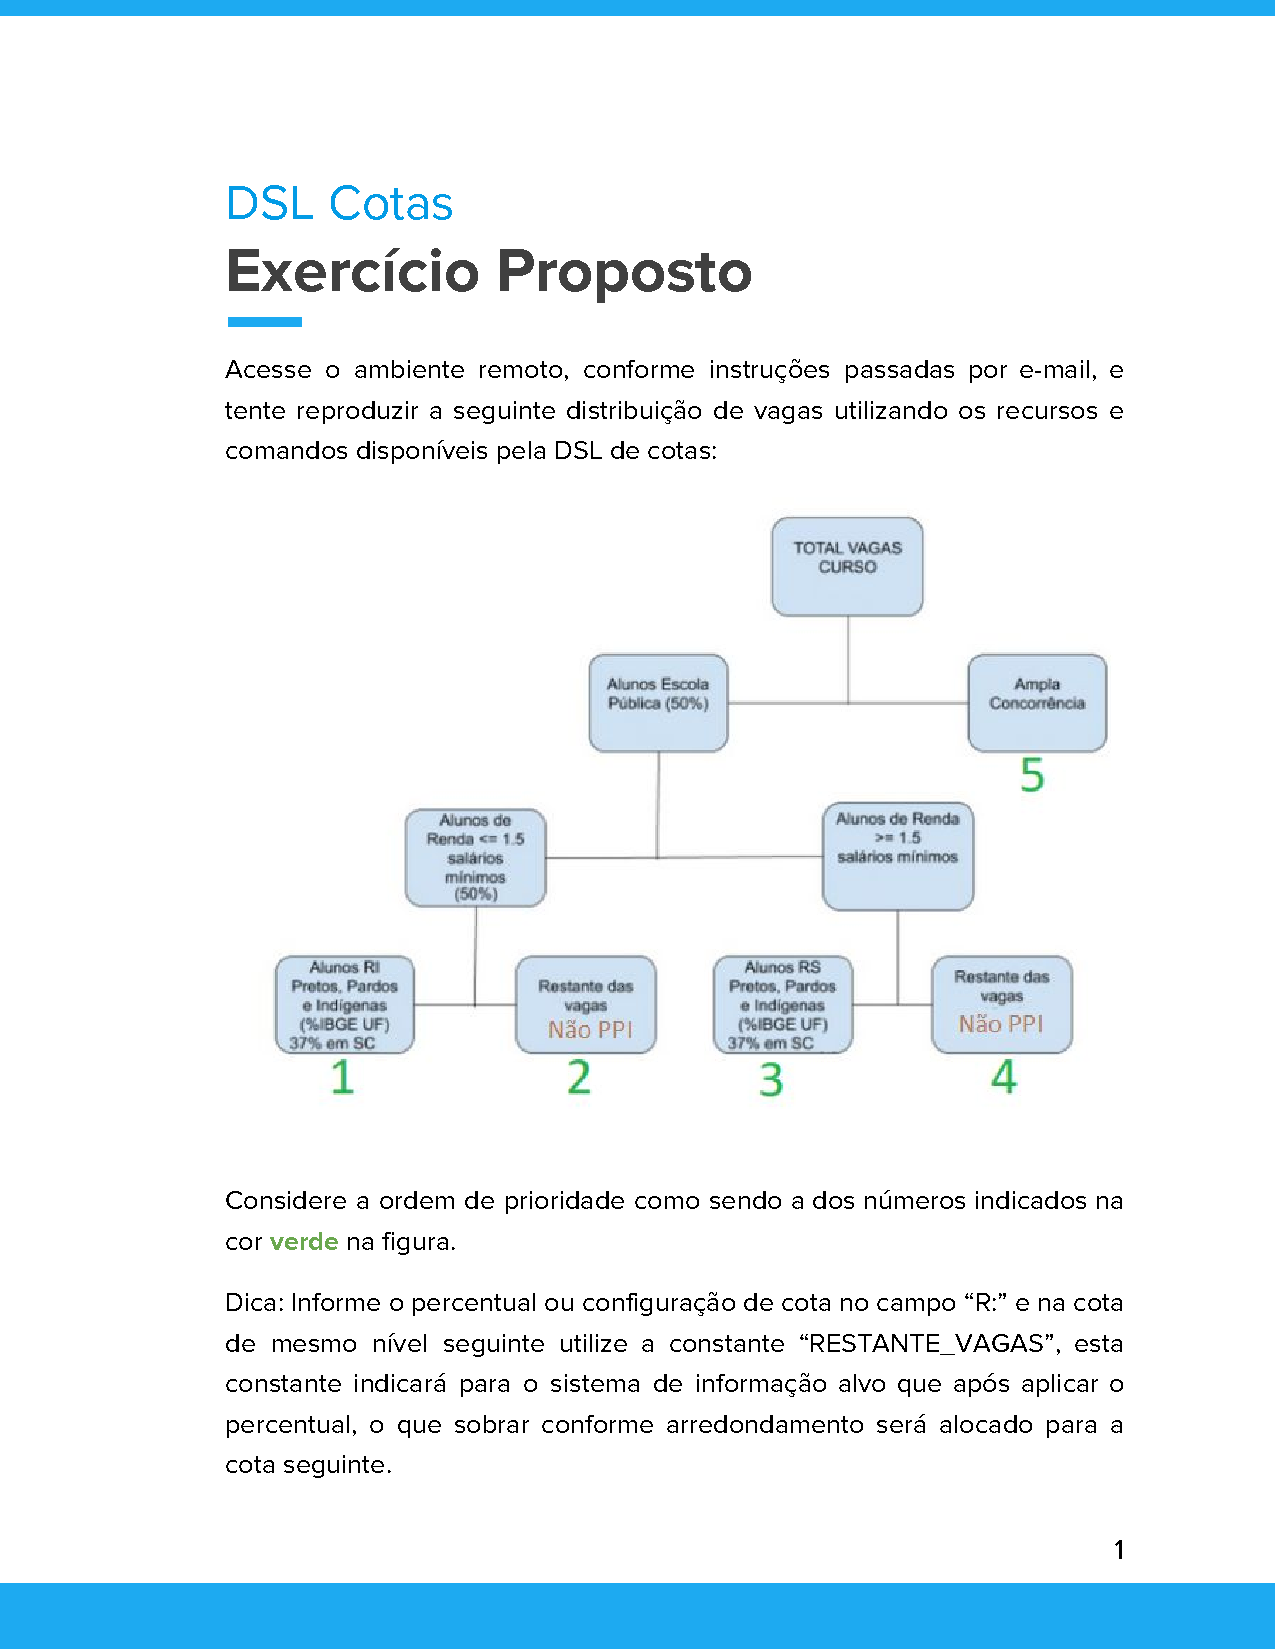
\includepdf[pages={1},scale=0.80,pagecommand=\chapter{Exercício de avaliação}\label{chap:apen:exercicio}]{appendix/TODOS/exerciciodslcotas}
\includepdf[pages={2},scale=0.80,pagecommand={}]{appendix/TODOS/exerciciodslcotas}

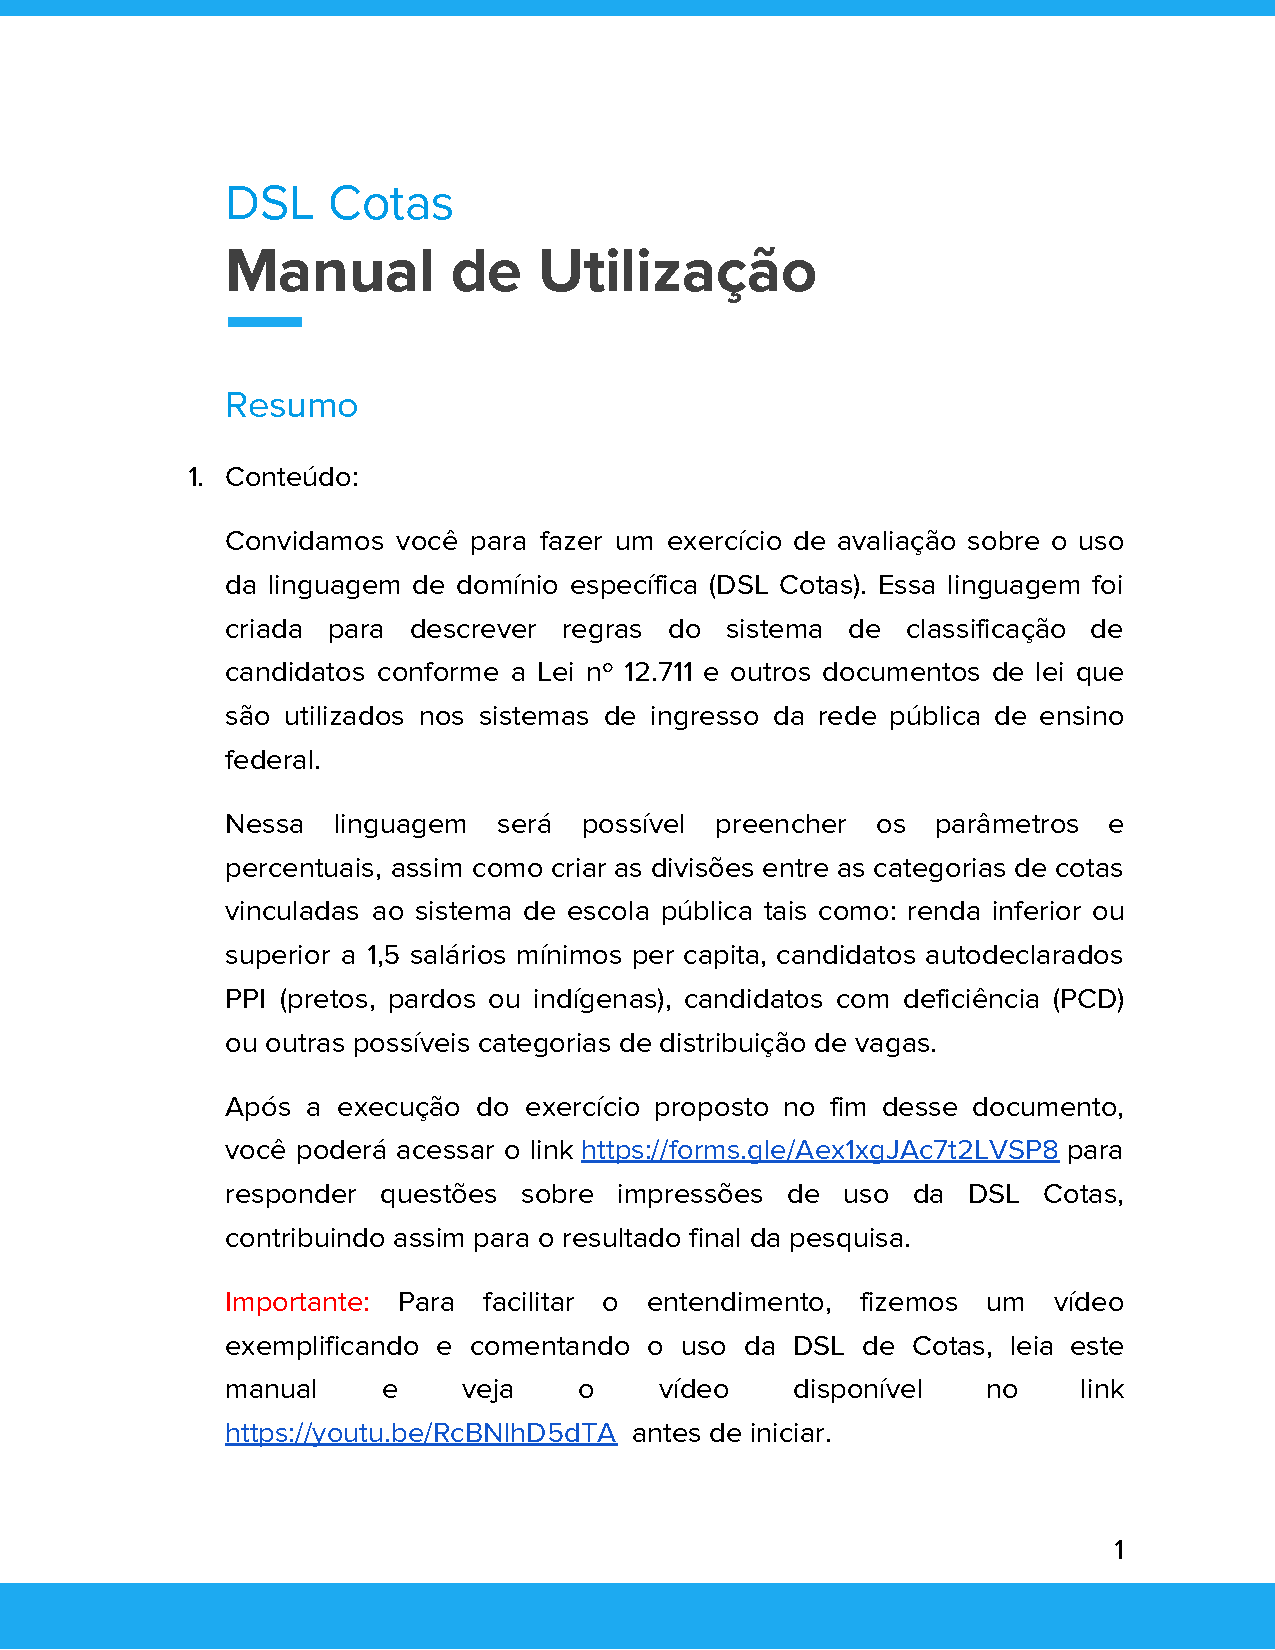
\includepdf[pages={1},scale=0.80,pagecommand=\chapter{Manual de utilização da DSL Cotas}\label{chap:apen:manual}]{appendix/TODOS/manualdslcotas}
\includepdf[pages={2-},scale=0.80,pagecommand={}]{appendix/TODOS/manualdslcotas}

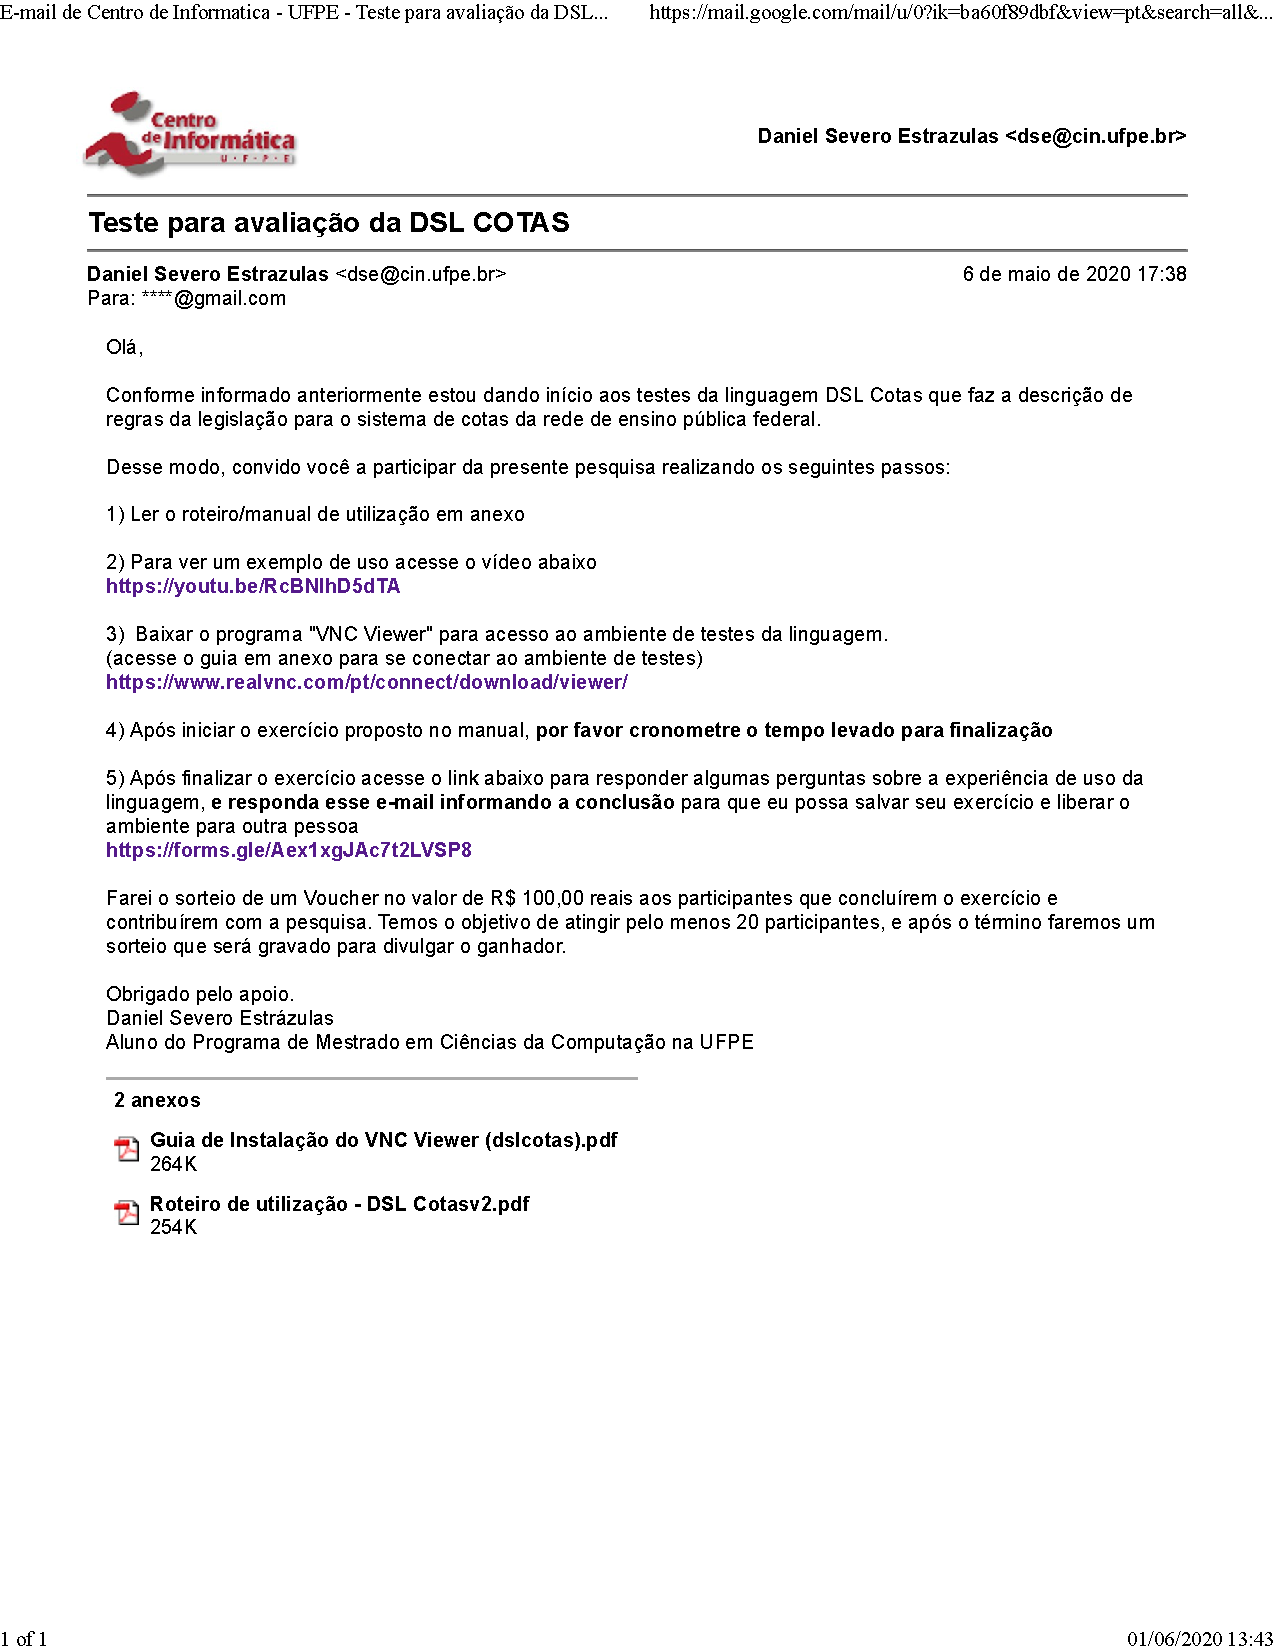
\includepdf[pages={1},scale=0.80,pagecommand=\chapter{E-mail para avaliação da pesquisa}\label{chap:apen:emaildslcotas}]{appendix/TODOS/emaildslcotas}


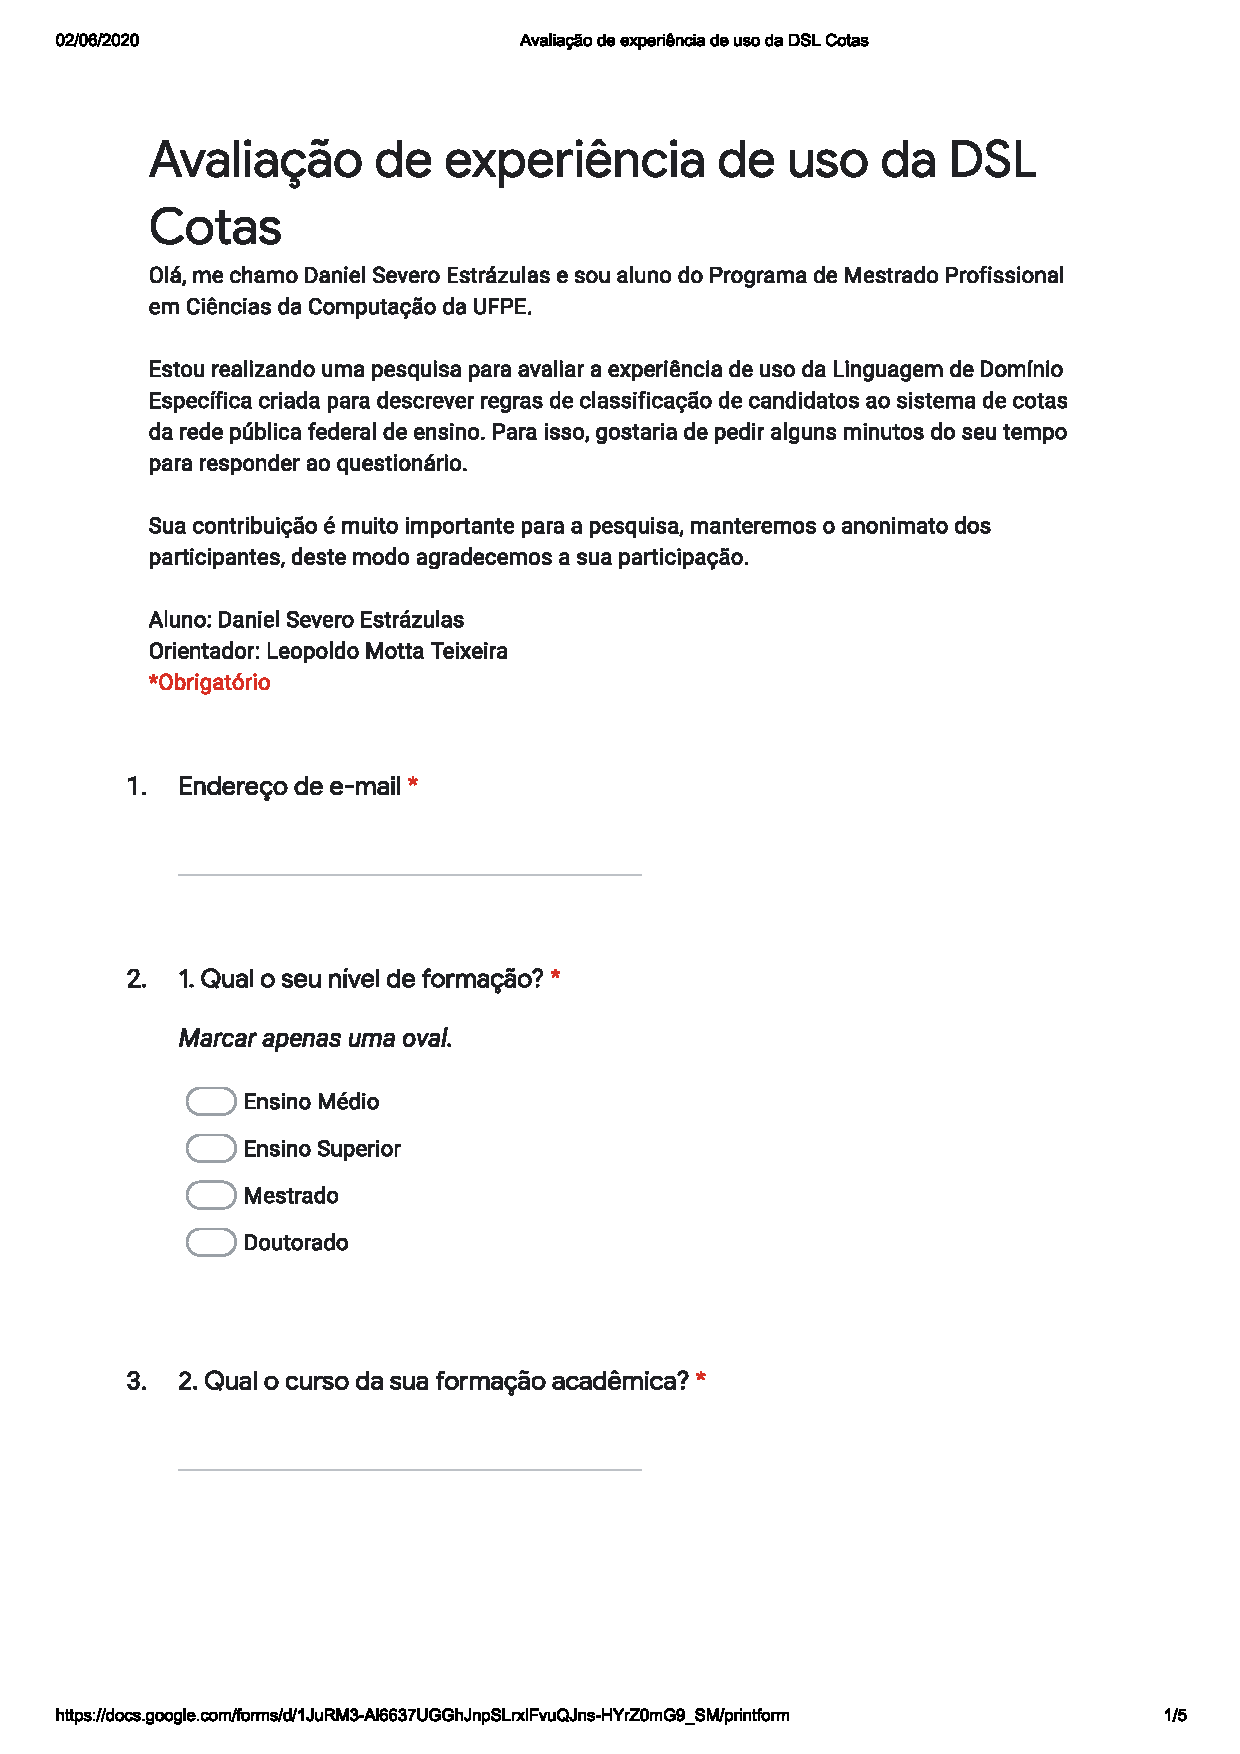
\includepdf[pages={1},scale=0.78,pagecommand=\chapter{Questionário de avaliação}\label{chap:apen:formularioapen}]{appendix/TODOS/formularioapen}
\includepdf[pages={2-},scale=0.80,pagecommand={}]{appendix/TODOS/formularioapen}

\addtocontents{toc}{\endgroup}
\end{apendicesenv}





\printindex


\end{document}
